\documentclass[12pt,a4paper]{report}

% =========================================================
% PACKAGES
% =========================================================

\usepackage[utf8]{inputenc}
\usepackage[T1]{fontenc}
\usepackage[french]{babel}

\usepackage{geometry}
\geometry{
    top=2.5cm,
    bottom=2.5cm,
    left=2.5cm,
    right=2.5cm
}

\usepackage{graphicx}
\usepackage{float}
\usepackage{xcolor}
\usepackage{listings}
\usepackage{hyperref}
\usepackage{enumitem}
\usepackage{array}
\usepackage{longtable}
\usepackage{booktabs}
\usepackage{fancyhdr}
\usepackage{titlesec}
% Supprimer le mot "Chapitre" des titres de chapitre
\titleformat{\chapter}
  {\normalfont\huge\bfseries}
  {\thechapter.}
  {1em}
  {}

% =========================================================
% CONFIGURATION
% =========================================================

\hypersetup{
    colorlinks=true,
    linkcolor=blue,
    urlcolor=blue,
    citecolor=blue
}

\pagestyle{fancy}
\fancyhf{}
\lhead{Documentation technique}
\rhead{Backend -- Parc Informatique}
\cfoot{\thepage}

% =========================================================
% CONFIGURATION DU CODE
% =========================================================

\definecolor{codegray}{rgb}{0.95,0.95,0.95}
\definecolor{codegreen}{rgb}{0.0,0.5,0.0}
\definecolor{codeblue}{rgb}{0.0,0.2,0.7}

\lstset{
    backgroundcolor=\color{codegray},
    basicstyle=\ttfamily\small,
    keywordstyle=\color{codeblue}\bfseries,
    commentstyle=\color{codegreen},
    stringstyle=\color{red},
    numbers=left,
    numberstyle=\tiny,
    numbersep=8pt,
    frame=single,
    breaklines=true,
    showstringspaces=false,
    tabsize=4
}

% =========================================================
% INFORMATIONS
% =========================================================

\title{
    \textbf{Documentation Technique du Backend}\\[0.5cm]
    \Large Plateforme de Gestion du Parc Informatique
}

\author{
Kaabachi Alaa
}


% =========================================================
% DOCUMENT
% =========================================================

\begin{document}

% ---------------------------------------------------------
% PAGE DE GARDE
% ---------------------------------------------------------

\maketitle

\begin{center}
    \vfill

    \textbf{Technologies utilisées}

    \vspace{0.3cm}

    FastAPI -- SQLAlchemy -- PostgreSQL -- Pydantic

    \vfill

    Documentation de la partie Backend
\end{center}

\thispagestyle{empty}

\newpage

% ---------------------------------------------------------
% TABLE DES MATIERES
% ---------------------------------------------------------

\tableofcontents

\newpage

% =========================================================
% 1. INTRODUCTION
% =========================================================

\chapter{Introduction}

Le backend de la plateforme de gestion du parc informatique a pour objectif
de fournir une API permettant de gérer les différents éléments du parc
informatique et les opérations associées.

La partie backend assure notamment :

\begin{itemize}
    \item la gestion des utilisateurs et des rôles ;
    \item la gestion des matériels informatiques ;
    \item la gestion des catégories et des emplacements ;
    \item la gestion des réparations et de leur historique ;
    \item la gestion des demandes d'achat, d'intervention et de support ;
    \item la communication avec la base de données PostgreSQL ;
    \item la validation des données échangées avec le frontend.
\end{itemize}

L'application backend est développée avec \textbf{FastAPI}, tandis que
\textbf{SQLAlchemy} est utilisé comme ORM pour communiquer avec PostgreSQL.

% =========================================================
% 2. ARCHITECTURE
% =========================================================

\{Architecture du Backend}

Le backend est organisé en plusieurs couches afin de séparer les
responsabilités et de faciliter la maintenance et l'évolution de
l'application.

La structure générale du projet est la suivante :

\begin{lstlisting}
app/
|
+-- main.py
|
+-- database/
|   +-- base.py
|   +-- connection.py
|   |
|   +-- models/
|       +-- role.py
|       +-- user.py
|       +-- material.py
|       +-- category.py
|       +-- location.py
|       +-- repair.py
|       +-- request.py
|
+-- schemas/
|   +-- role.py
|   +-- user.py
|   +-- material.py
|   +-- category.py
|   +-- location.py
|   +-- repair.py
|   +-- request.py
|
+-- routers/
    +-- roles.py
    +-- users.py
    +-- materials.py
    +-- categories.py
    +-- locations.py
    +-- repairs.py
    +-- requests.py
\end{lstlisting}

\begin{figure}[H]
    \centering
    % Remplacer par le nom réel de votre image
    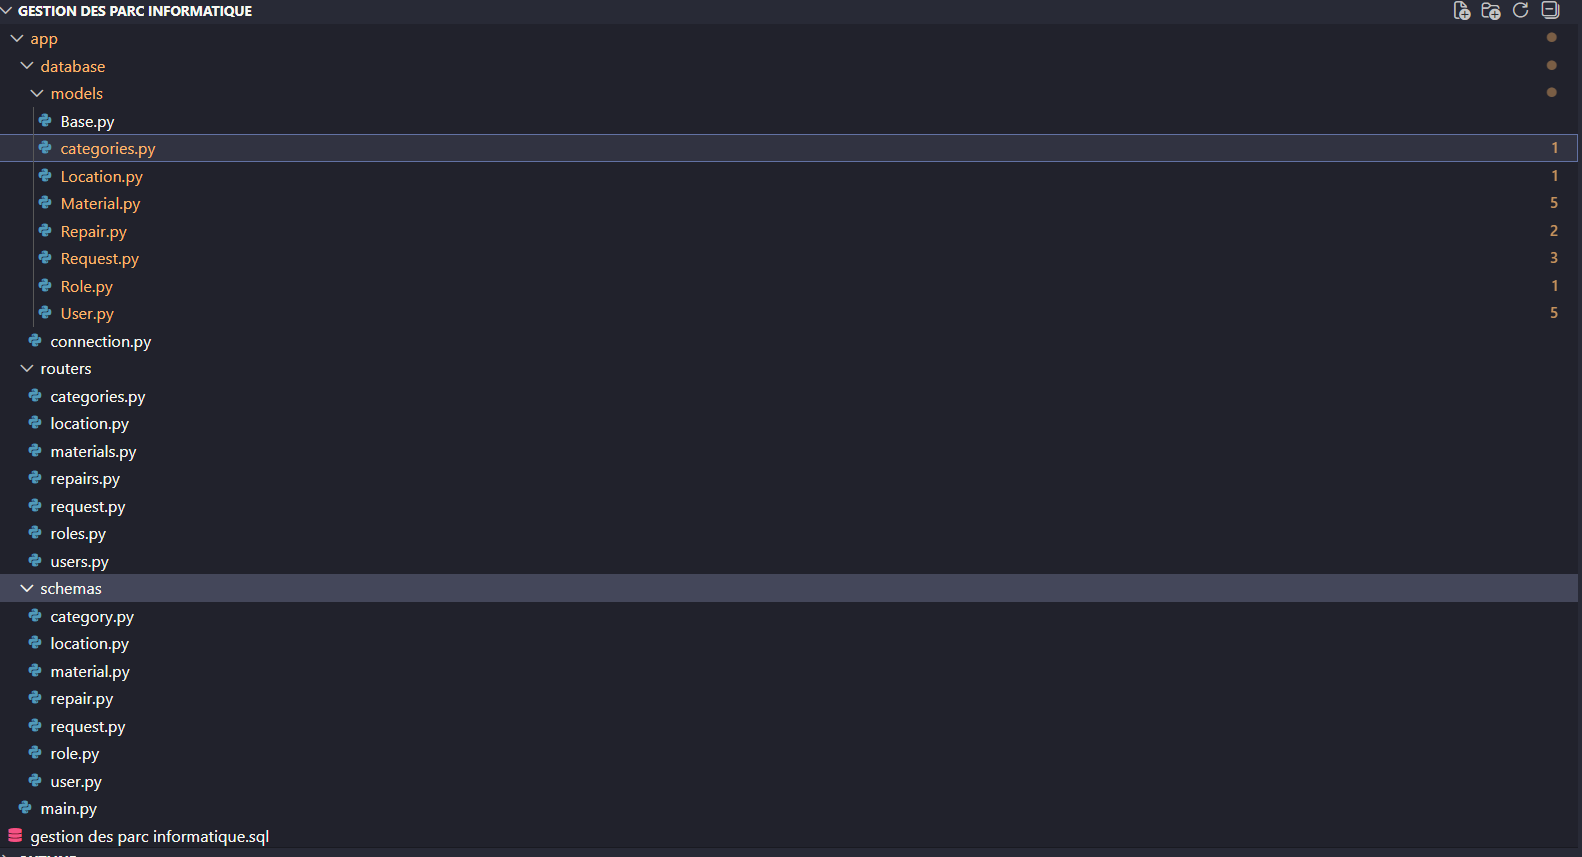
\includegraphics[width=0.8\textwidth]{screenshots/architecture.png}


\end{figure}

Cette organisation permet de séparer :

\begin{itemize}
    \item la connexion à la base de données ;
    \item les modèles SQLAlchemy ;
    \item les schémas Pydantic ;
    \item les routes FastAPI ;
    \item le point d'entrée de l'application.
\end{itemize}

% =========================================================
% 3. CONNEXION DATABASE
% =========================================================

\chapter{Connexion à PostgreSQL}

La communication avec PostgreSQL est réalisée à l'aide de SQLAlchemy.

Le fichier \texttt{connection.py} contient les paramètres nécessaires à la
connexion ainsi que la création de l'Engine et des sessions.



La variable \texttt{DATABASE\_URL} contient les informations nécessaires
pour accéder à la base de données :

\begin{itemize}
    \item \texttt{postgresql+psycopg} : PostgreSQL avec le driver Psycopg ;
    \item \texttt{postgres} : utilisateur PostgreSQL ;
    \item \texttt{localhost} : serveur local ;
    \item \texttt{5432} : port PostgreSQL ;
    \item \texttt{parc\_informatique} : nom de la base de données.
\end{itemize}

La fonction \texttt{create\_engine()} crée l'Engine SQLAlchemy qui permet
de gérer les connexions vers PostgreSQL.

\begin{figure}[H]
    \centering
    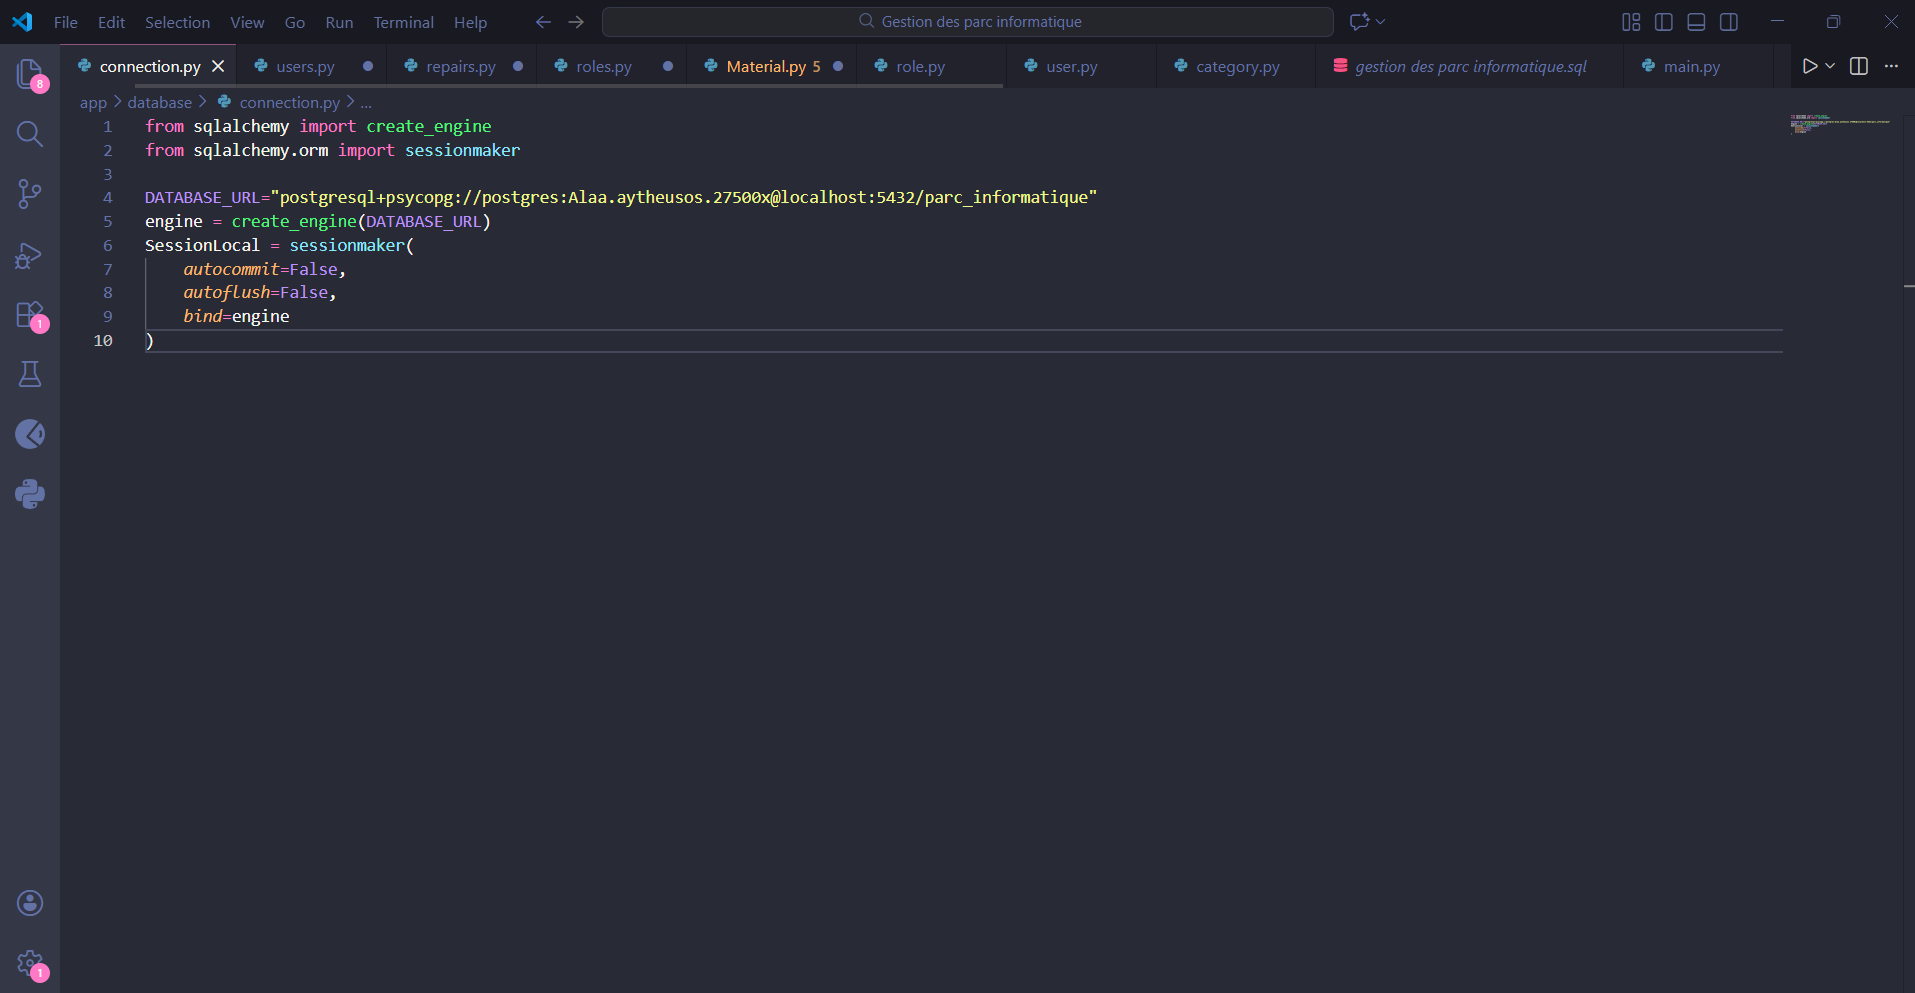
\includegraphics[width=0.8\textwidth]{screenshots/connection.png}
    \caption{Configuration de la connexion PostgreSQL}
    \label{fig:connection}
\end{figure}

\textbf{Remarque de sécurité :} le mot de passe réel de la base de données
ne doit pas être exposé dans le rapport ou dans un dépôt Git public. Il est
préférable d'utiliser des variables d'environnement.

% =========================================================
% 4. SESSION
% =========================================================

\section{Gestion des sessions}

Une fonction \texttt{get\_db()} est utilisée afin de créer une session pour
chaque requête puis de la fermer une fois l'opération terminée.



Le fonctionnement est donc :

\begin{center}
\textbf{
Requête HTTP
$\rightarrow$
get\_db()
$\rightarrow$
Session
$\rightarrow$
PostgreSQL
$\rightarrow$
Fermeture de la session
}
\end{center}

\begin{figure}[H]
    \centering
    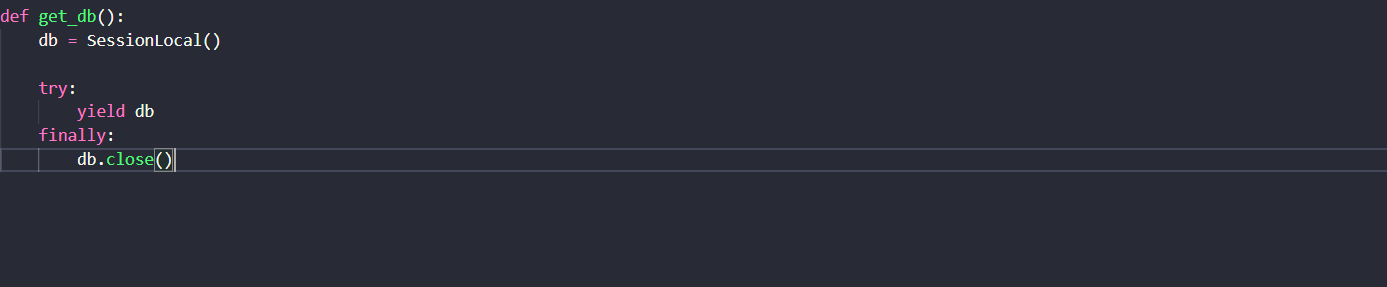
\includegraphics[width=0.8\textwidth]{screenshots/get_db.png}
    \caption{Gestion des sessions SQLAlchemy}
    \label{fig:getdb}
\end{figure}

% =========================================================
% 5. BASE
% =========================================================

\chapter{Base déclarative SQLAlchemy}

Une classe \texttt{Base} commune est utilisée par les différents modèles
SQLAlchemy.

\begin{lstlisting}[language=Python]
from sqlalchemy.orm import DeclarativeBase

class Base(DeclarativeBase):
    pass
\end{lstlisting}

Les modèles héritent ensuite de cette classe :

\begin{lstlisting}[language=Python]
class User(Base):
    __tablename__ = "users"
\end{lstlisting}

Cela indique à SQLAlchemy que la classe \texttt{User} représente une table
de la base de données.

\begin{figure}[H]
    \centering
    \begin{figure}[H]
    \centering
    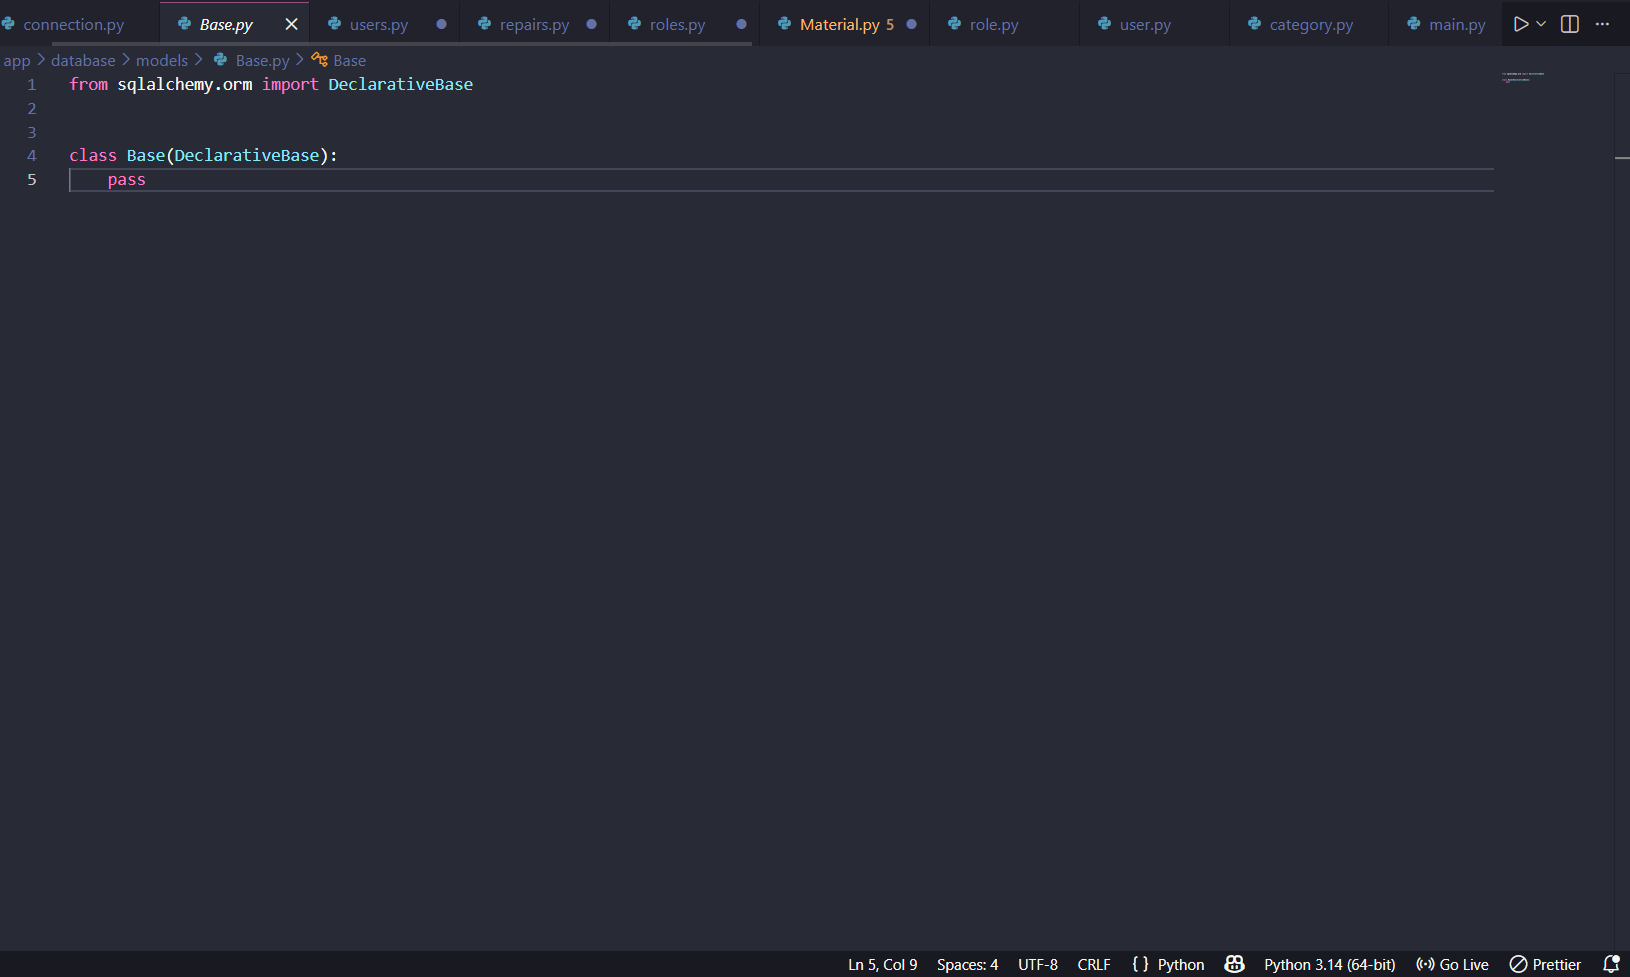
\includegraphics[width=0.8\textwidth]{screenshots/base.png}
    \caption{Gestion des sessions SQLAlchemy}
    \label{fig:getdb}
\end{figure}
    \caption{Classe déclarative Base}
    \label{fig:base}
\end{figure}

% =========================================================
% 6. MODELISATION
% =========================================================

\chapter{Modélisation des données}

Les tables PostgreSQL sont représentées par des classes Python grâce à
SQLAlchemy.

Les colonnes sont déclarées à l'aide de \texttt{Mapped} et
\texttt{mapped\_column()}.

Par exemple :

\begin{lstlisting}[language=Python]
id: Mapped[int] = mapped_column(
    primary_key=True
)
\end{lstlisting}

représente une clé primaire.

% =========================================================
% 7. ROLE
% =========================================================

\section{Modèle Role}

Le modèle \texttt{Role} représente les rôles disponibles dans la
plateforme.

\begin{lstlisting}[language=Python]
class Role(Base):
    __tablename__ = "roles"

    id: Mapped[int] = mapped_column(
        primary_key=True
    )

    name: Mapped[str] = mapped_column(
        String(50),
        unique=True,
        nullable=False
    )

    description: Mapped[str | None] = mapped_column(
        Text
    )

    users: Mapped[list["User"]] = relationship(
        back_populates="role"
    )
\end{lstlisting}

Le champ \texttt{name} est unique afin d'éviter l'existence de deux rôles
ayant le même nom.

La relation \texttt{users} permet d'accéder aux utilisateurs associés à
un rôle.


\begin{figure}[H]
    \centering
    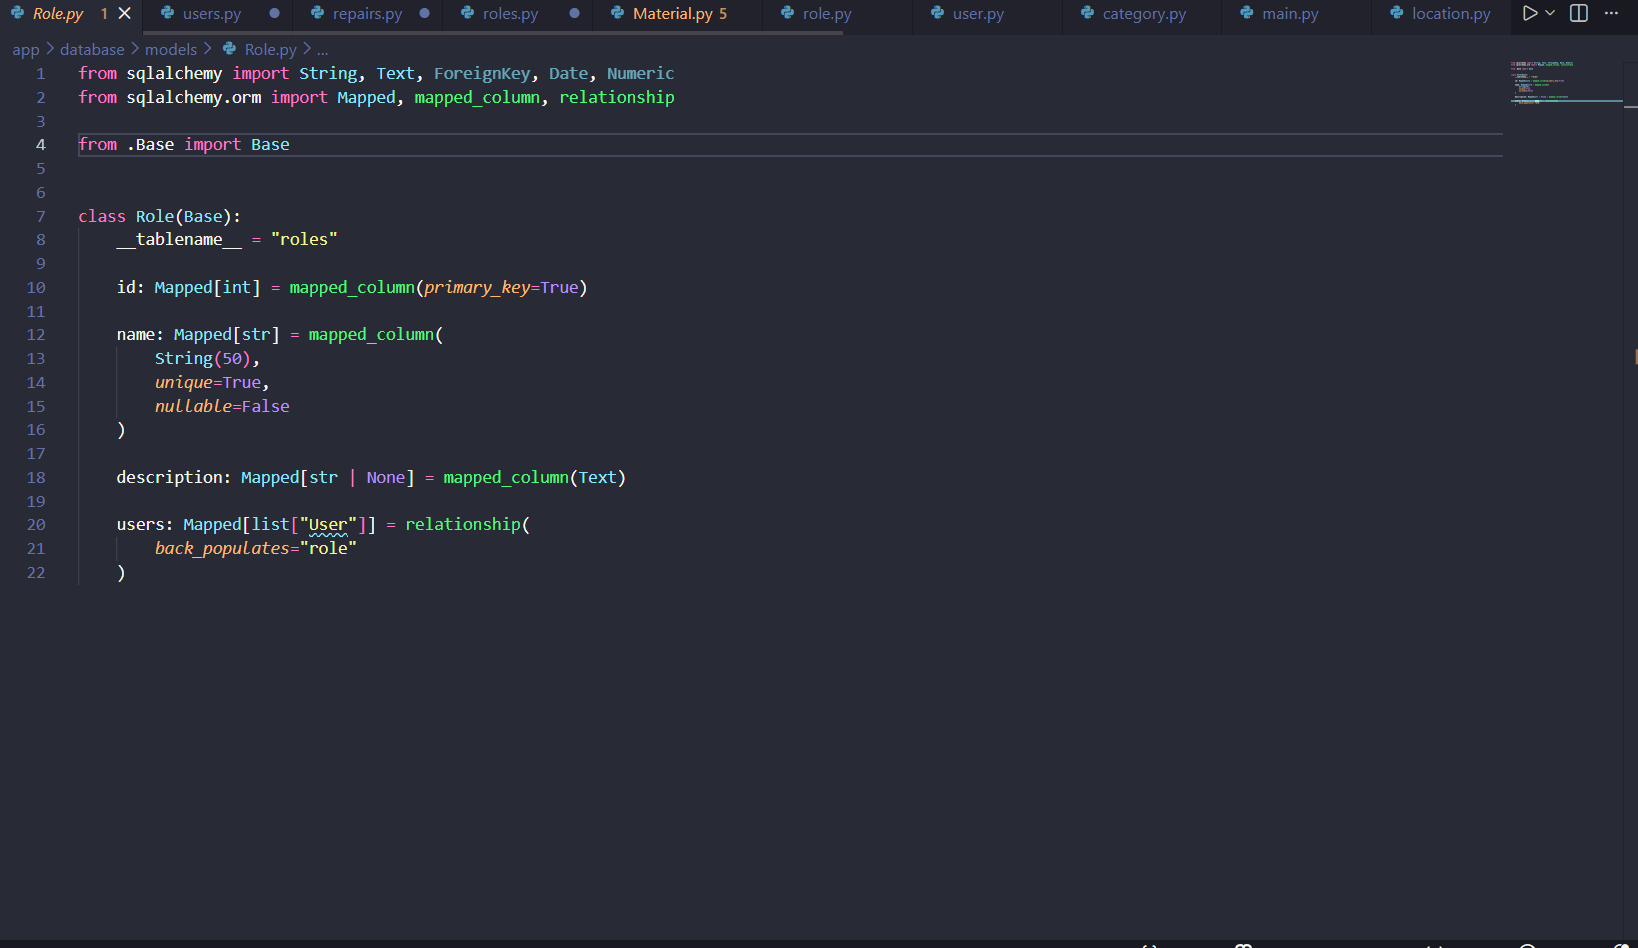
\includegraphics[width=0.8\textwidth]{screenshots/role.png}
    \caption{Gestion des sessions SQLAlchemy}
    \label{fig:getdb}
\end{figure}

% =========================================================
% 8. USER
% =========================================================

\section{Modèle User}

Le modèle \texttt{User} représente les utilisateurs de la plateforme.

Il contient notamment :

\begin{itemize}
    \item username ;
    \item first\_name ;
    \item last\_name ;
    \item email ;
    \item password\_hash ;
    \item role\_id ;
    \item is\_active.
\end{itemize}

\begin{lstlisting}[language=Python]
class User(Base):
    __tablename__ = "users"

    id: Mapped[int] = mapped_column(
        primary_key=True
    )

    username: Mapped[str] = mapped_column(
        String(100),
        unique=True,
        nullable=False
    )

    first_name: Mapped[str] = mapped_column(
        String(100),
        nullable=False
    )

    last_name: Mapped[str] = mapped_column(
        String(100),
        nullable=False
    )

    email: Mapped[str] = mapped_column(
        String(255),
        unique=True,
        nullable=False
    )

    password_hash: Mapped[str] = mapped_column(
        Text,
        nullable=False
    )

    role_id: Mapped[int] = mapped_column(
        ForeignKey("roles.id"),
        nullable=False
    )

    is_active: Mapped[bool] = mapped_column(
        default=True,
        nullable=False
    )
\end{lstlisting}

\begin{figure}[H]
    \centering
    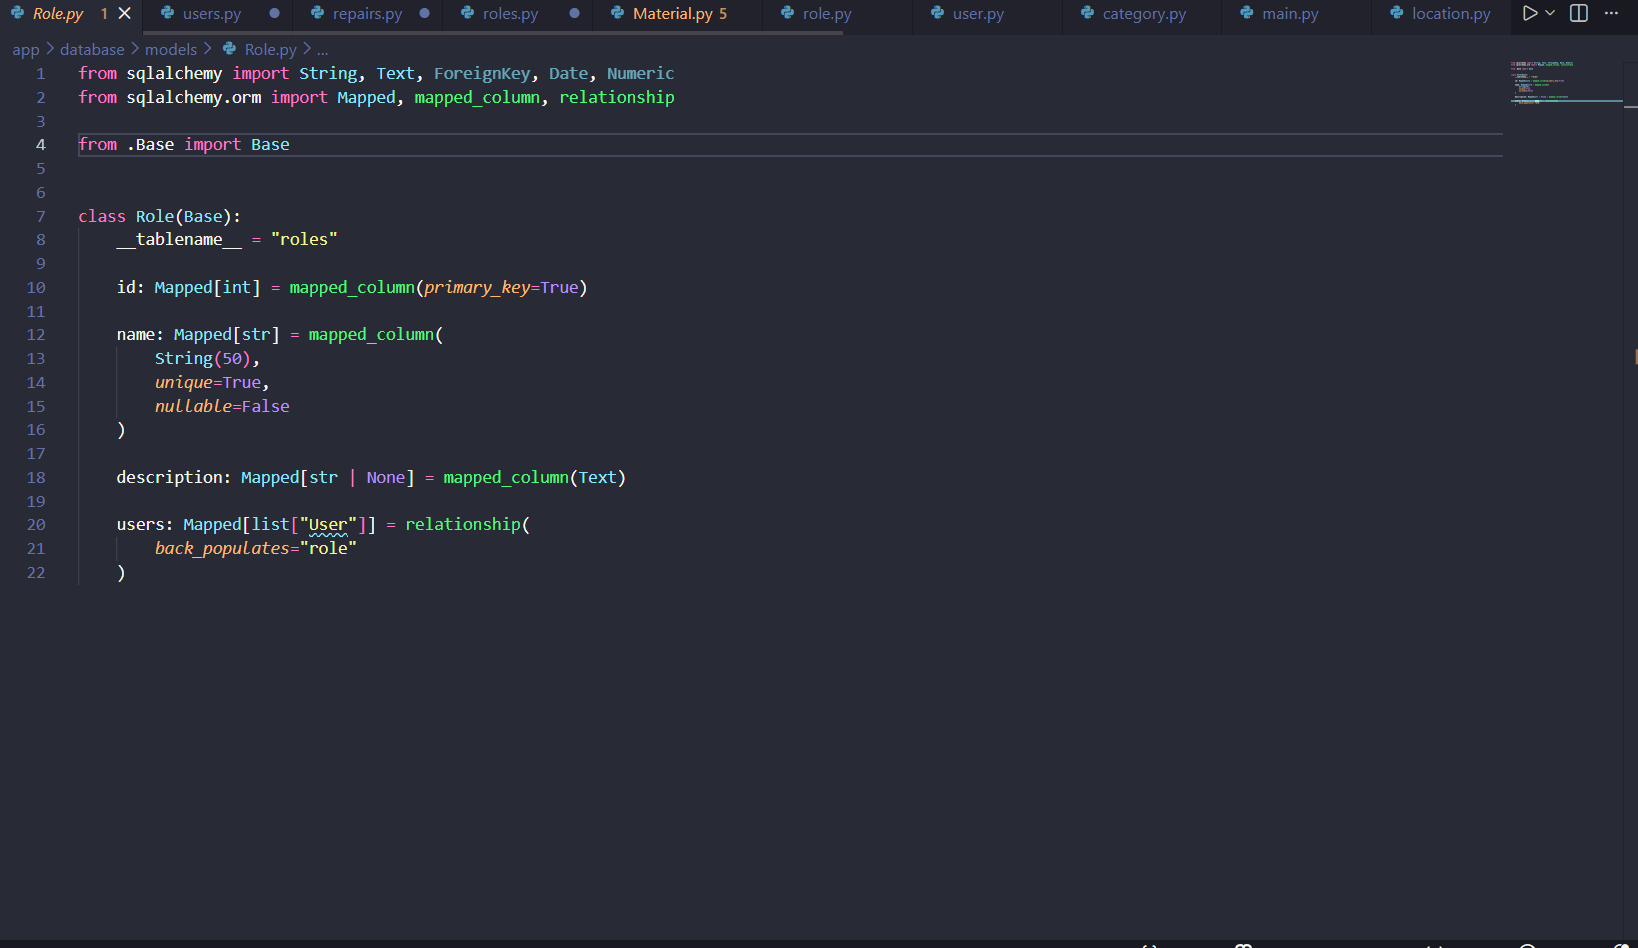
\includegraphics[width=0.8\textwidth]{screenshots/role.png}
    \caption{Gestion des sessions SQLAlchemy}
    \label{fig:getdb}
\end{figure}

% =========================================================
% 9. RELATIONS USER
% =========================================================

\section{Relations du modèle User}

Le modèle \texttt{User} possède plusieurs relations.

\subsection{Relation avec Role}

\begin{lstlisting}[language=Python]
role: Mapped["Role"] = relationship(
    back_populates="users"
)
\end{lstlisting}

Cette relation permet notamment d'utiliser :

\begin{lstlisting}[language=Python]
user.role
\end{lstlisting}

La relation inverse permet :

\begin{lstlisting}[language=Python]
role.users
\end{lstlisting}

\subsection{Relation avec Material}

\begin{lstlisting}[language=Python]
materials: Mapped[list["Material"]] = relationship(
    back_populates="assigned_user"
)
\end{lstlisting}

Cette relation permet de récupérer les matériels affectés à un utilisateur.

\subsection{Relation avec Repair}

\begin{lstlisting}[language=Python]
repairs: Mapped[list["Repair"]] = relationship(
    back_populates="technician"
)
\end{lstlisting}

Cette relation permet de récupérer les réparations prises en charge par
un technicien.

\subsection{Relations avec Request}

Le modèle possède deux relations avec \texttt{Request}.

\begin{lstlisting}[language=Python]
created_requests: Mapped[list["Request"]] = relationship(
    back_populates="creator",
    foreign_keys="Request.created_by"
)

assigned_requests: Mapped[list["Request"]] = relationship(
    back_populates="assigned_to_user",
    foreign_keys="Request.assigned_to"
)
\end{lstlisting}

Cette distinction est nécessaire car une demande possède deux références
vers la table des utilisateurs :

\begin{itemize}
    \item \texttt{created\_by} : utilisateur qui crée la demande ;
    \item \texttt{assigned\_to} : utilisateur auquel la demande est affectée.
\end{itemize}
\section{Model Role}
\begin{figure}[H]
    \centering
    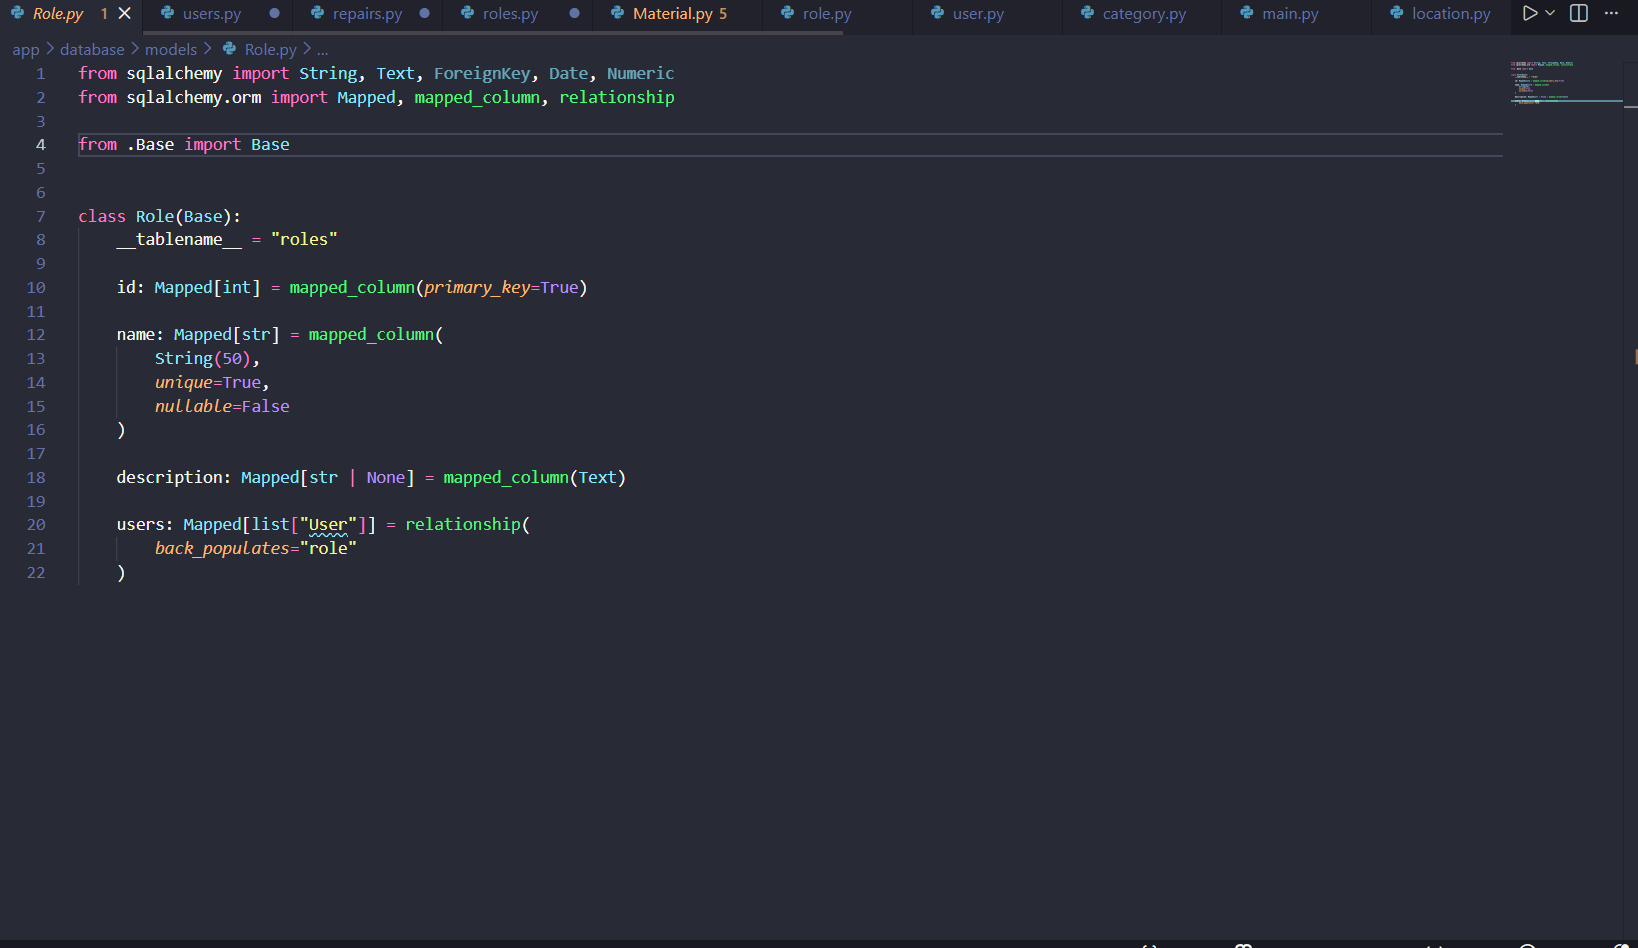
\includegraphics[width=0.8\textwidth]{screenshots/role.png}
    \caption{Role Model}
    \label{fig:getdb}
\end{figure}
\section{model user}
\begin{figure}[H]
    \centering
    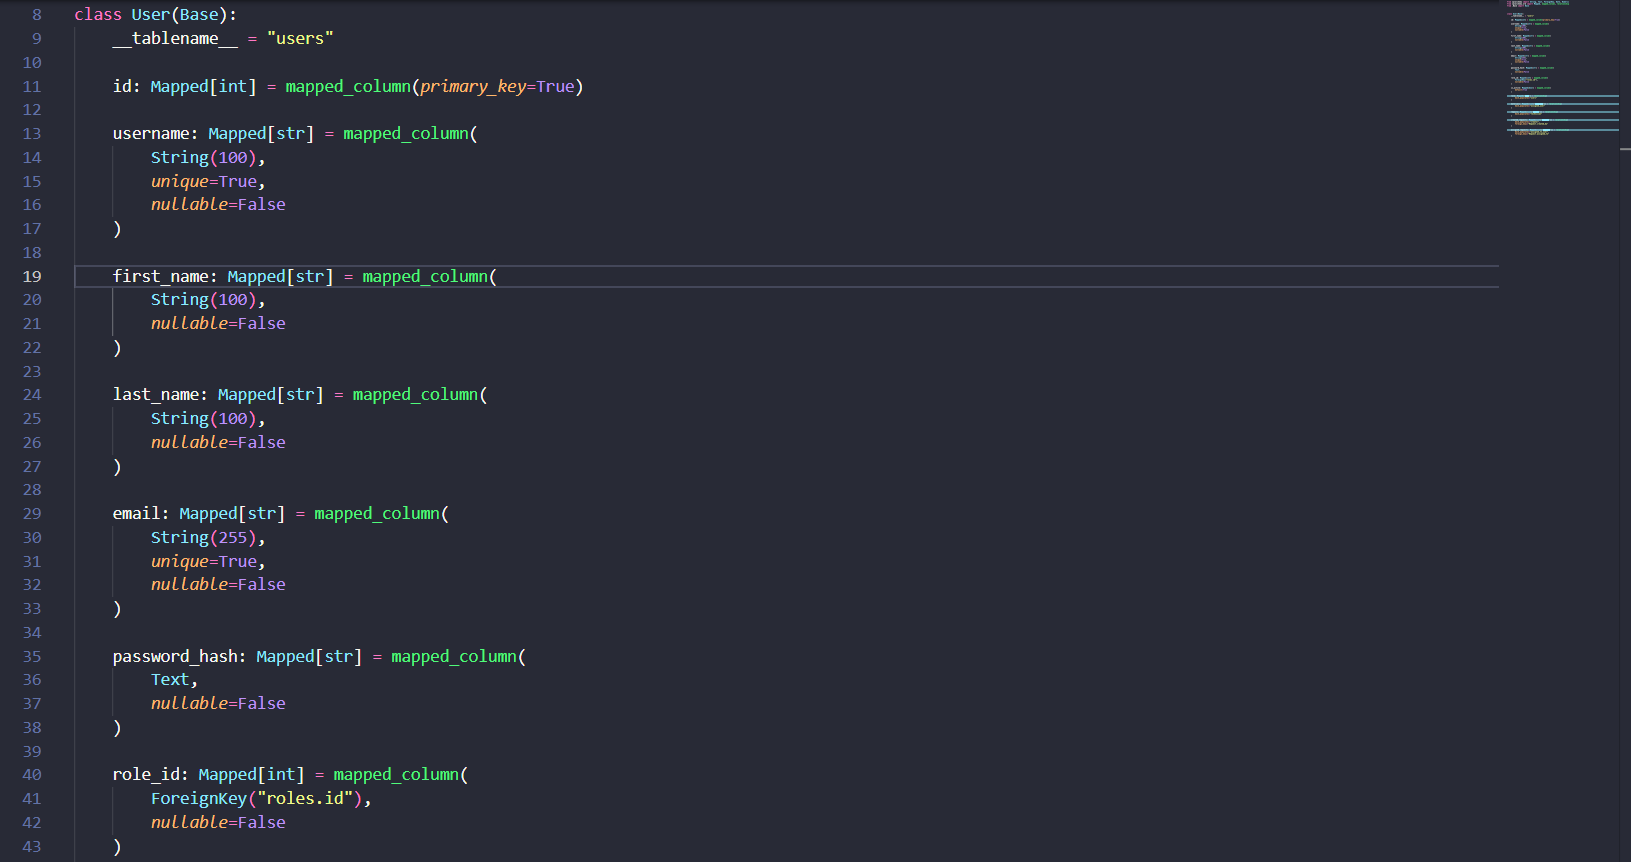
\includegraphics[width=0.8\textwidth]{screenshots/user.png}
    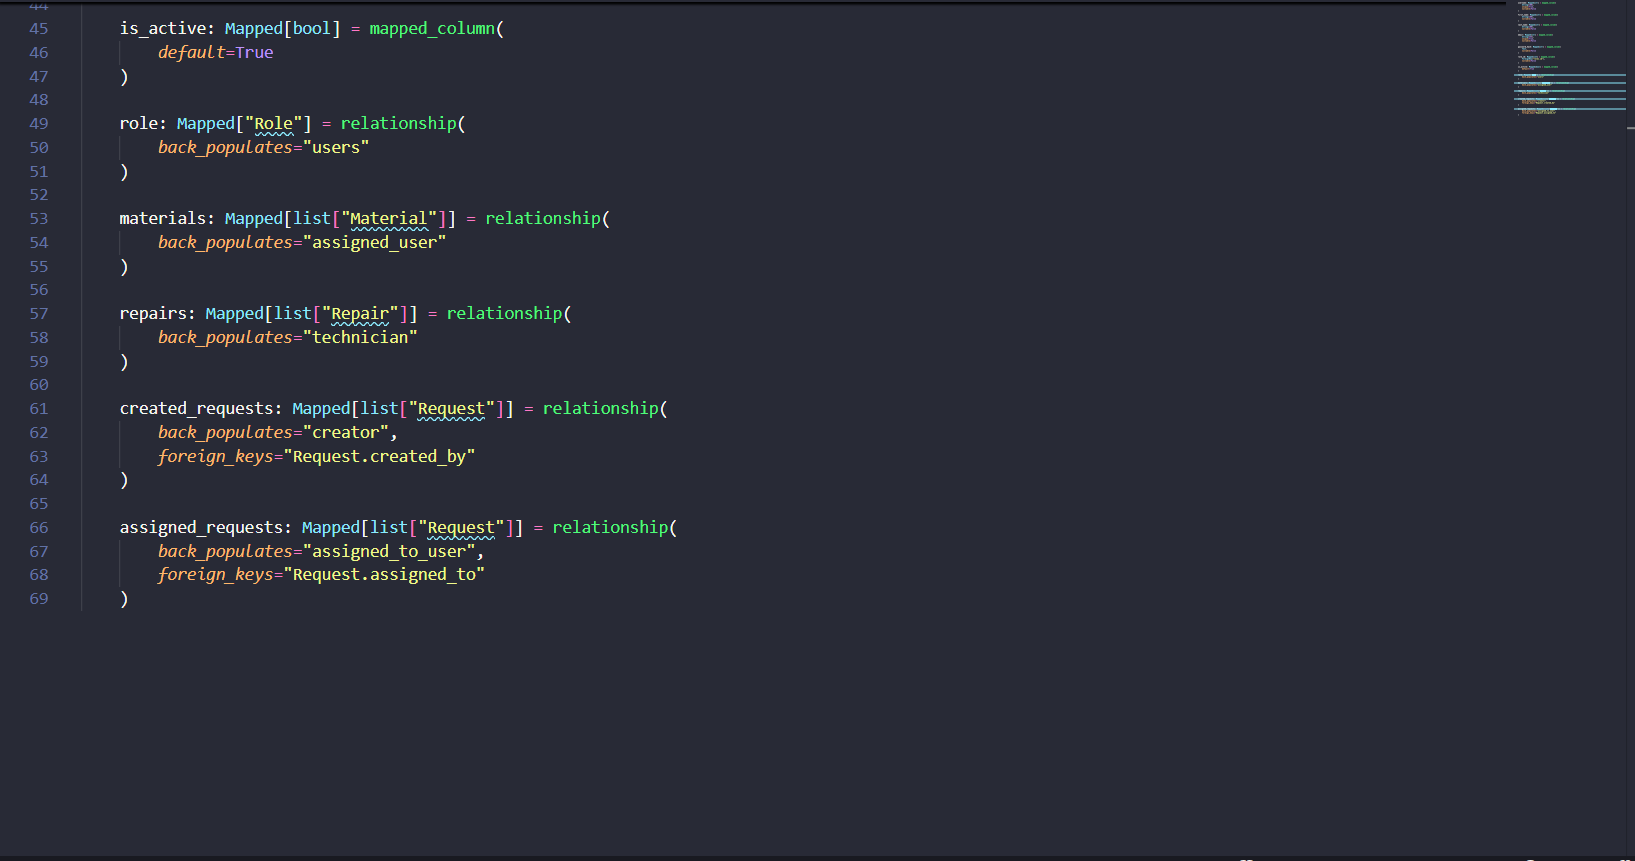
\includegraphics[width=0.8\textwidth]{screenshots/user1.png}
    \caption{Gestion des sessions SQLAlchemy}
    \label{fig:getdb}
\end{figure}

% =========================================================
% 10. FOREIGN KEY
% =========================================================



\section{Modèle Material}

Le modèle \texttt{Material} représente les équipements informatiques.

Il permet notamment de gérer :

\begin{itemize}
    \item l'identification du matériel ;
    \item sa catégorie ;
    \item son emplacement ;
    \item l'utilisateur auquel il est affecté ;
    \item son état.
\end{itemize}

\begin{figure}[H]
    \centering
    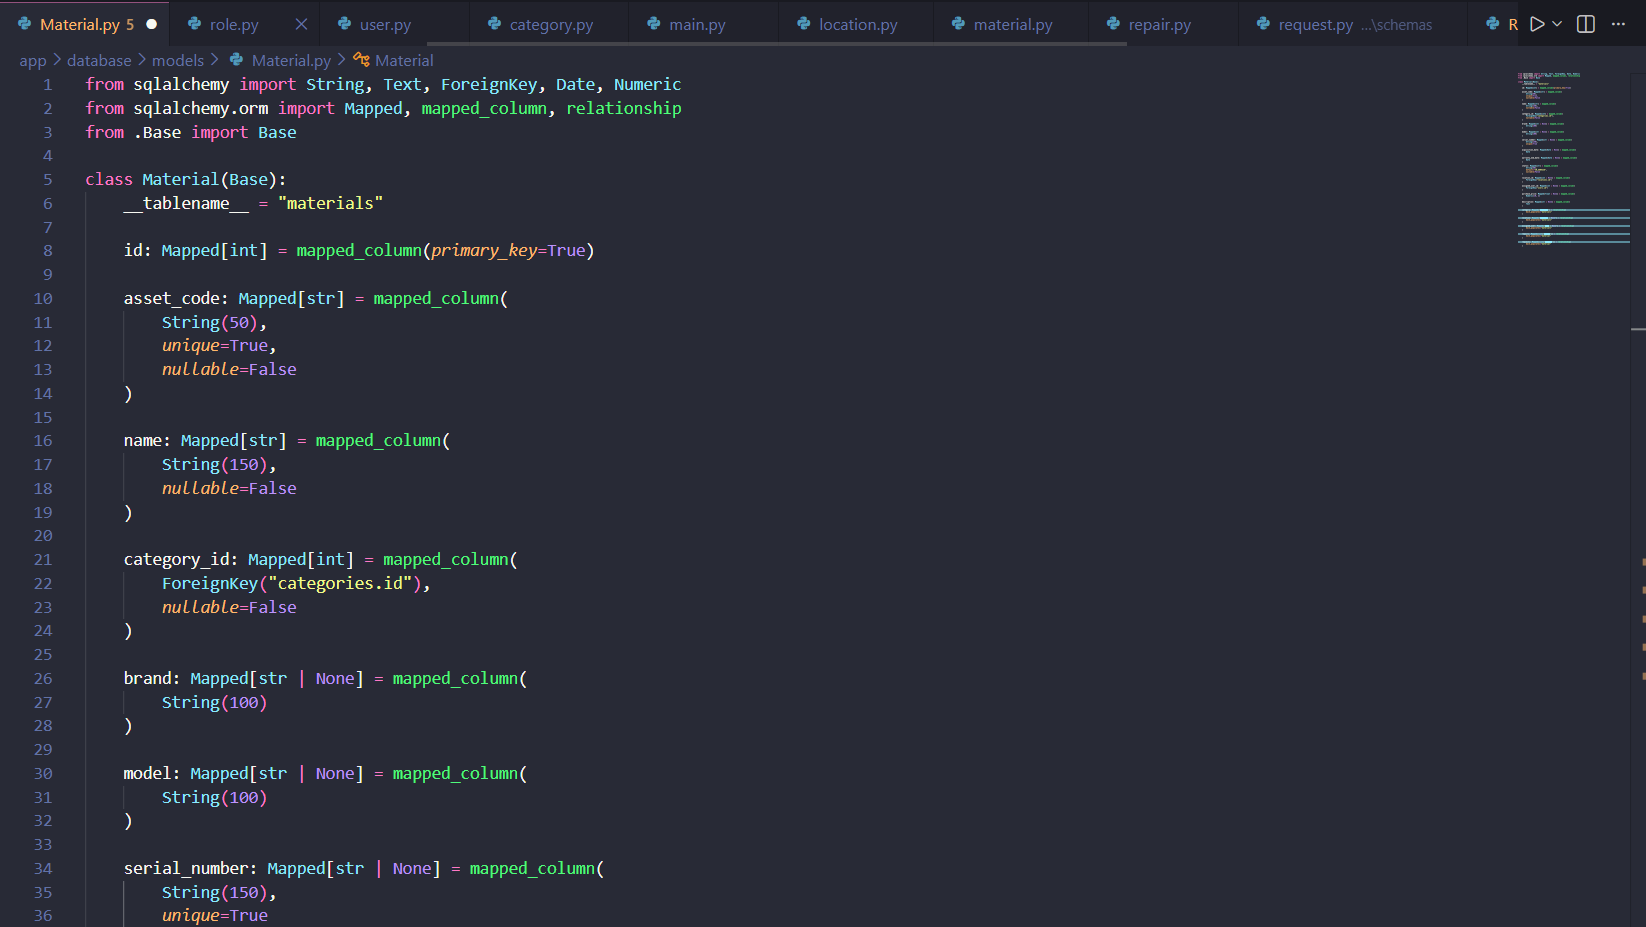
\includegraphics[width=0.8\textwidth]{screenshots/material.png}
    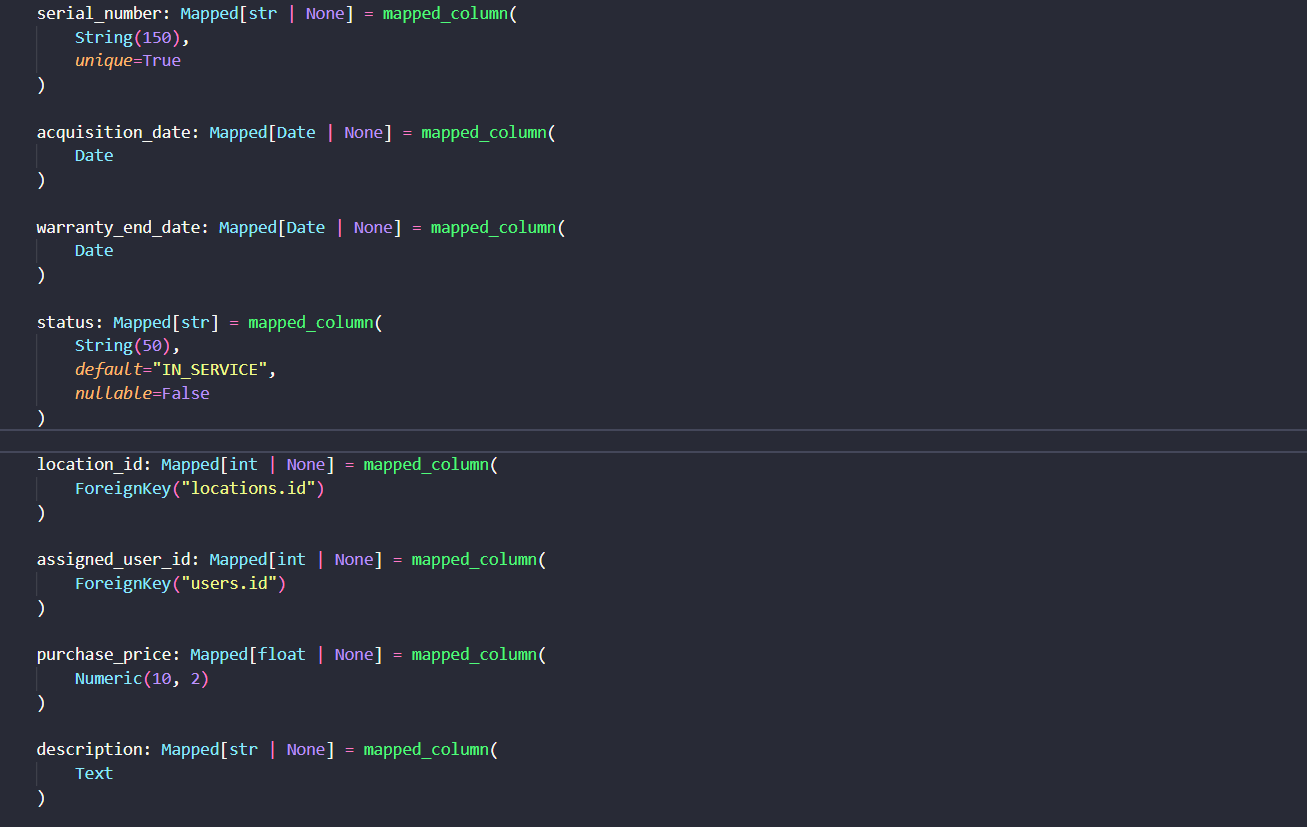
\includegraphics[width=0.8\textwidth]{screenshots/material1.png}
    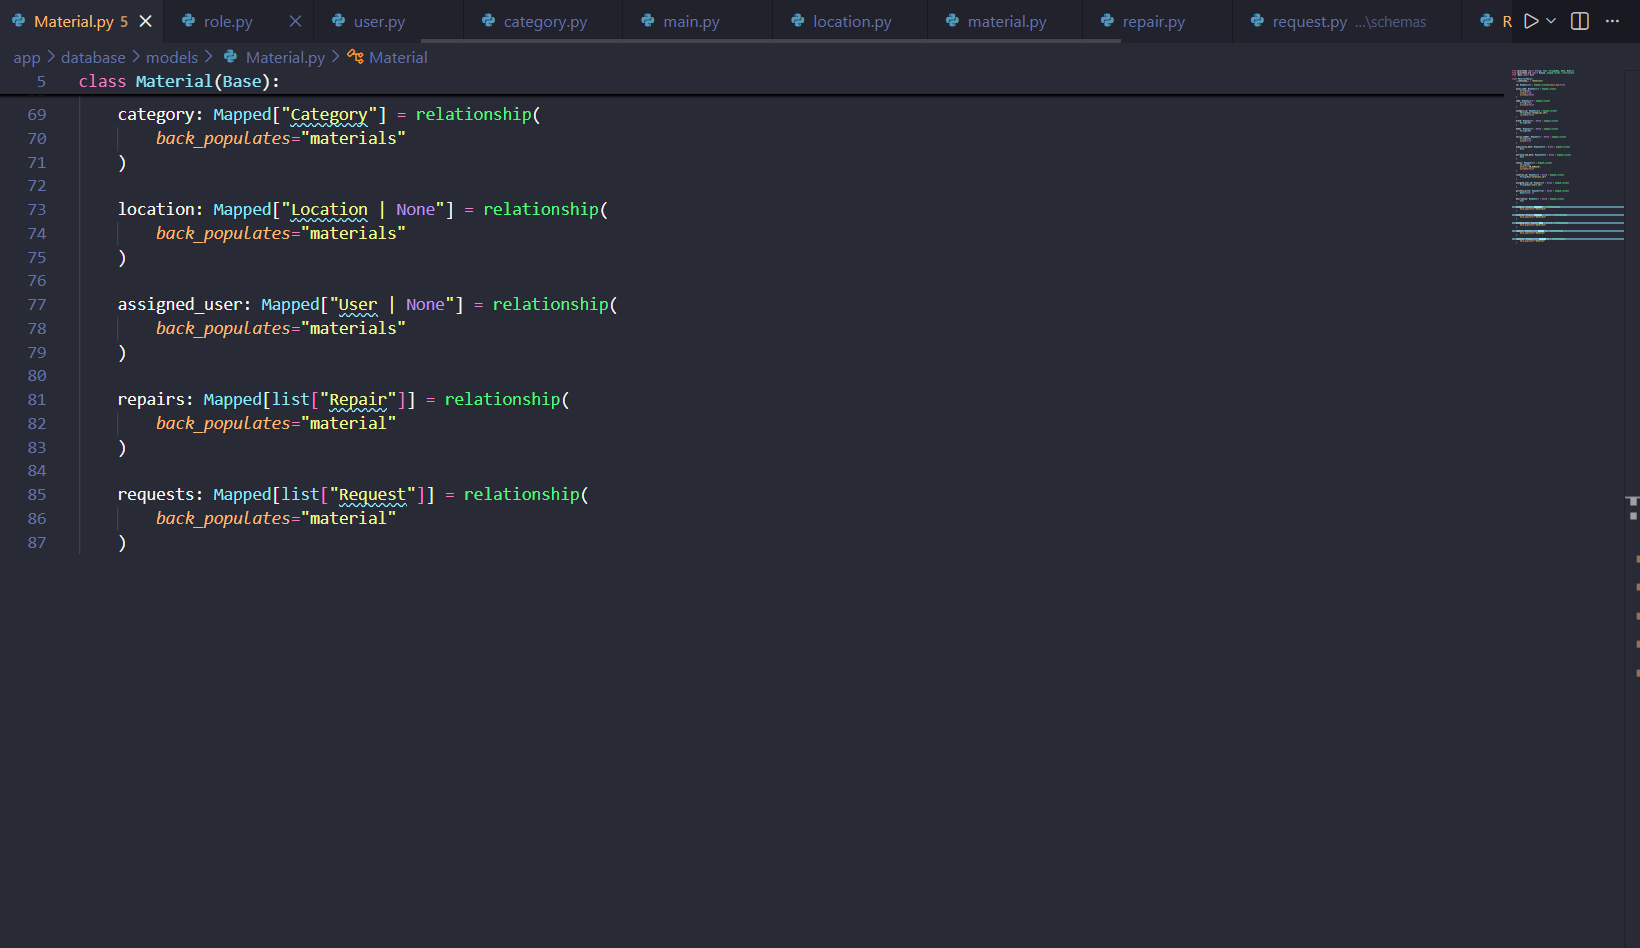
\includegraphics[width=0.8\textwidth]{screenshots/material2.png}
    \caption{Modèle Material}
\end{figure}

\section{Modèle Category}

Le modèle \texttt{Category} permet de classer les matériels informatiques.

\begin{figure}[H]
    \centering
    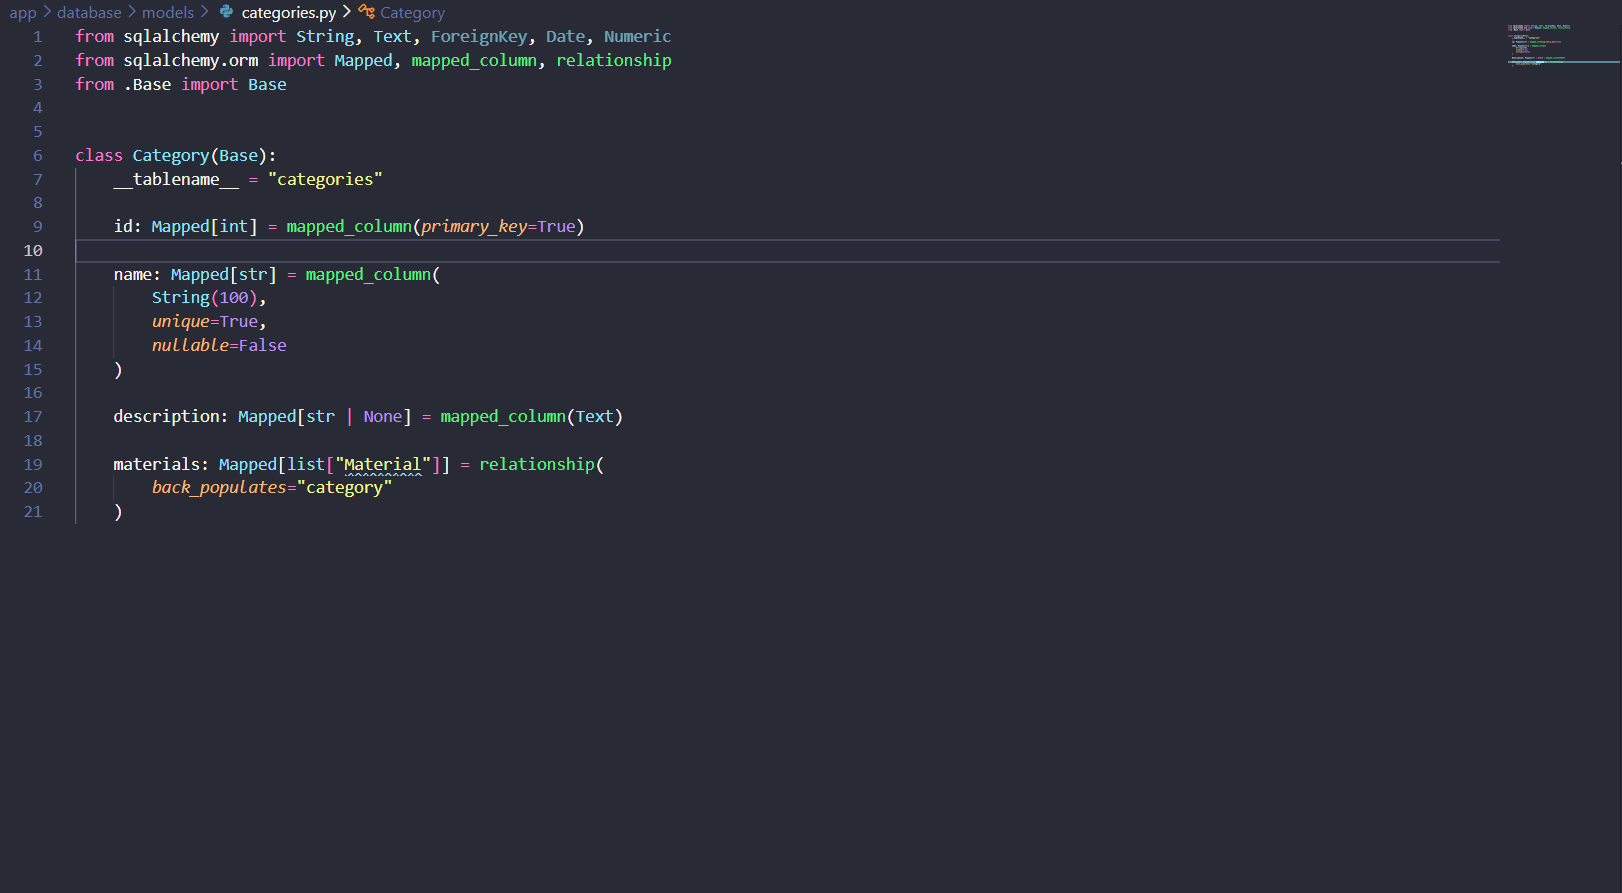
\includegraphics[width=0.8\textwidth]{screenshots/categories.png}
    \caption{Modèle Category}
\end{figure}

\section{Modèle Location}

Le modèle \texttt{Location} permet de gérer les emplacements des matériels.

\begin{figure}[H]
    \centering
    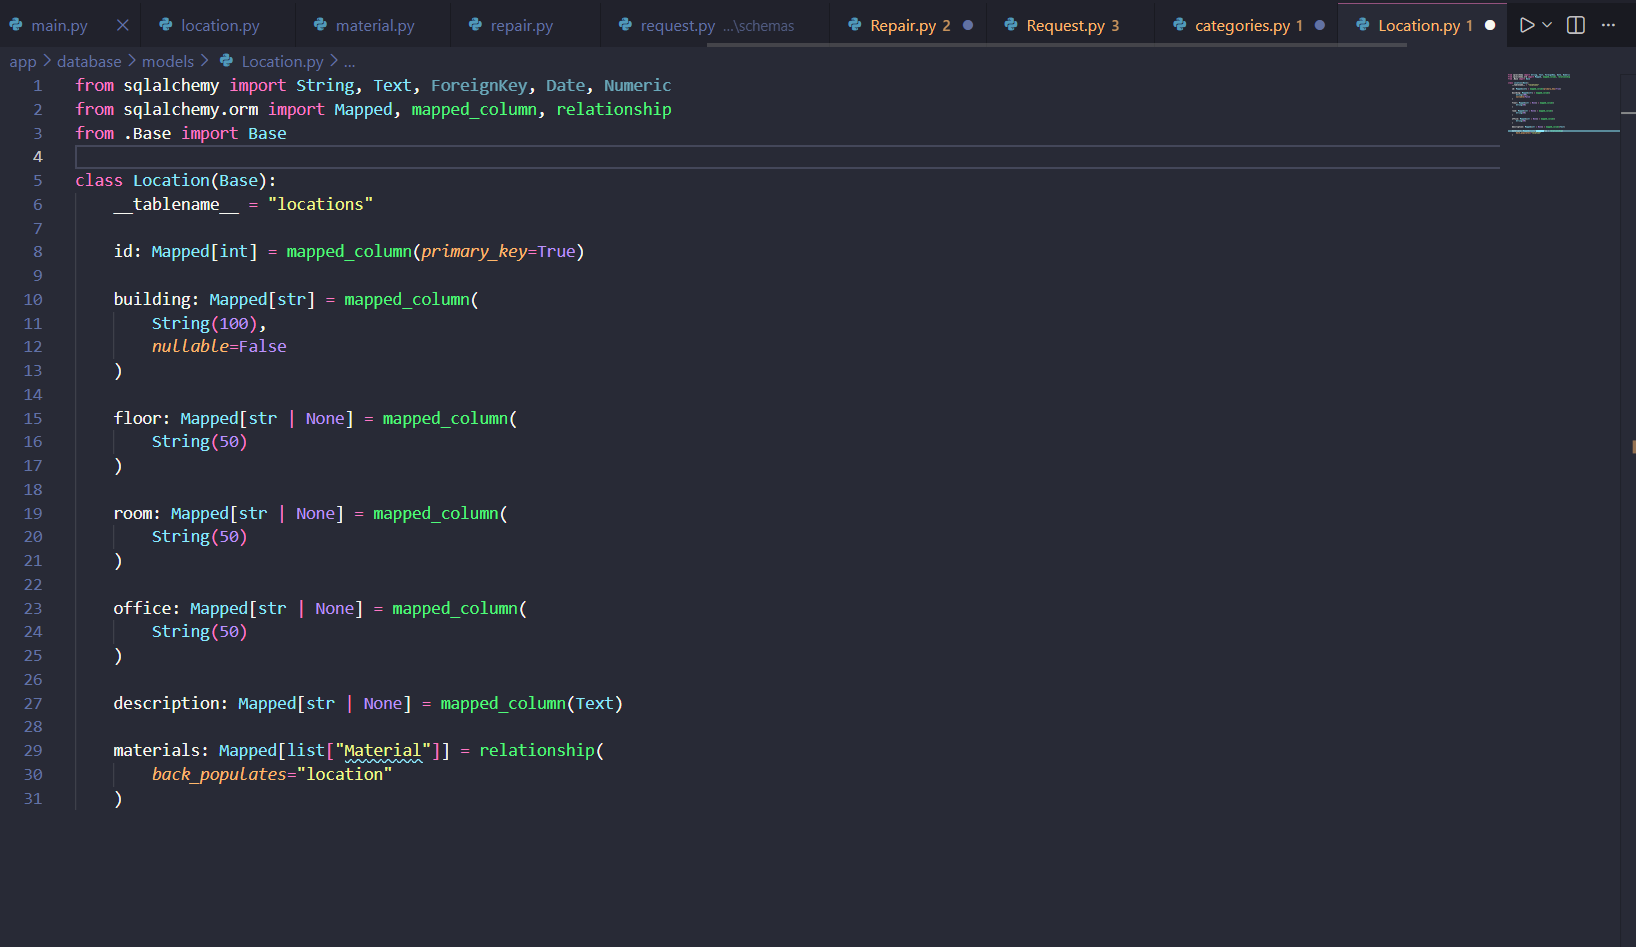
\includegraphics[width=0.8\textwidth]{screenshots/location.png}
    \caption{Modèle Location}
\end{figure}

\section{Modèle Repair}

Le modèle \texttt{Repair} permet de gérer les opérations de réparation.

Il constitue également la base de la fonctionnalité d'historique des
réparations d'un matériel.

\begin{figure}[H]
    \centering
    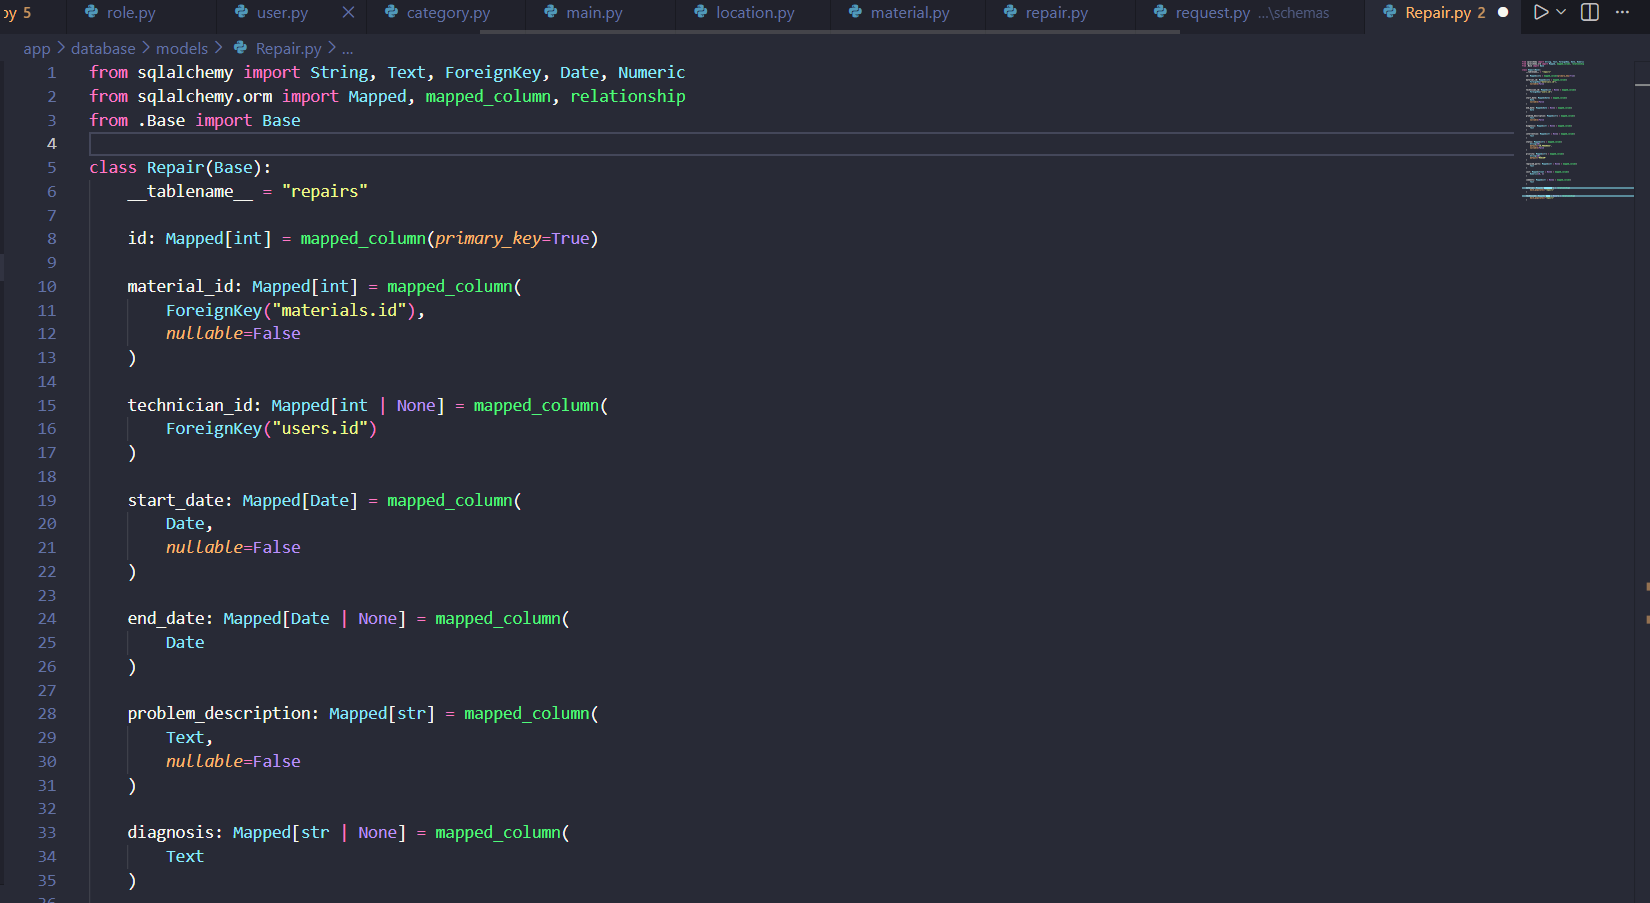
\includegraphics[width=0.8\textwidth]{screenshots/repair.png}
    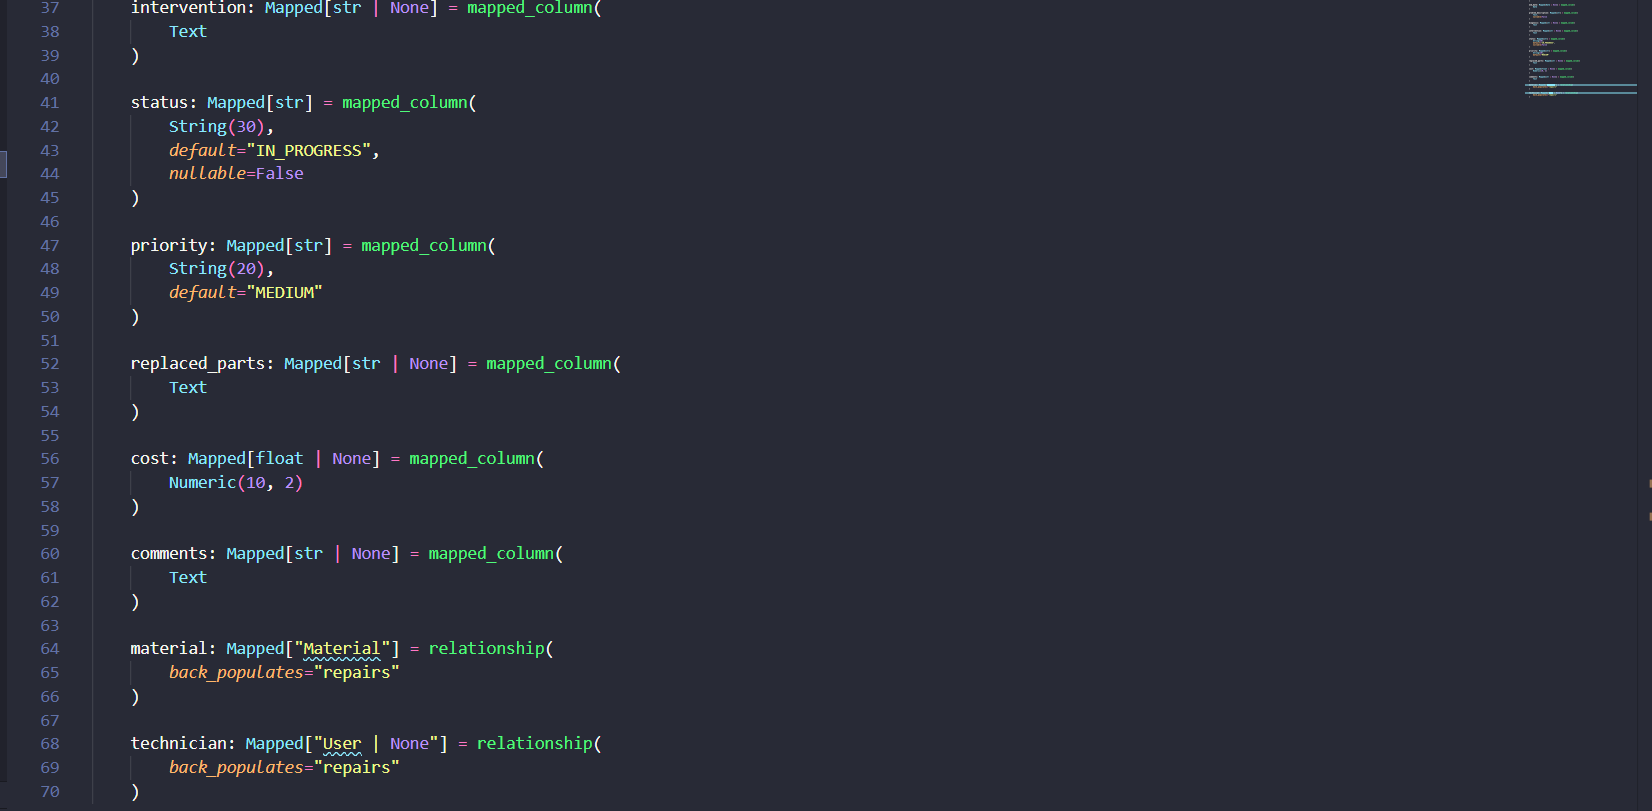
\includegraphics[width=0.8\textwidth]{screenshots/repair1.png}
    \caption{Modèle Repair}
\end{figure}

\section{Modèle Request}

Le modèle \texttt{Request} représente les différentes demandes effectuées
par les utilisateurs.

Les demandes peuvent notamment concerner :

\begin{itemize}
    \item une demande d'achat ;
    \item une demande d'intervention ;
    \item une demande de support.
\end{itemize}

\begin{figure}[H]
    \centering
    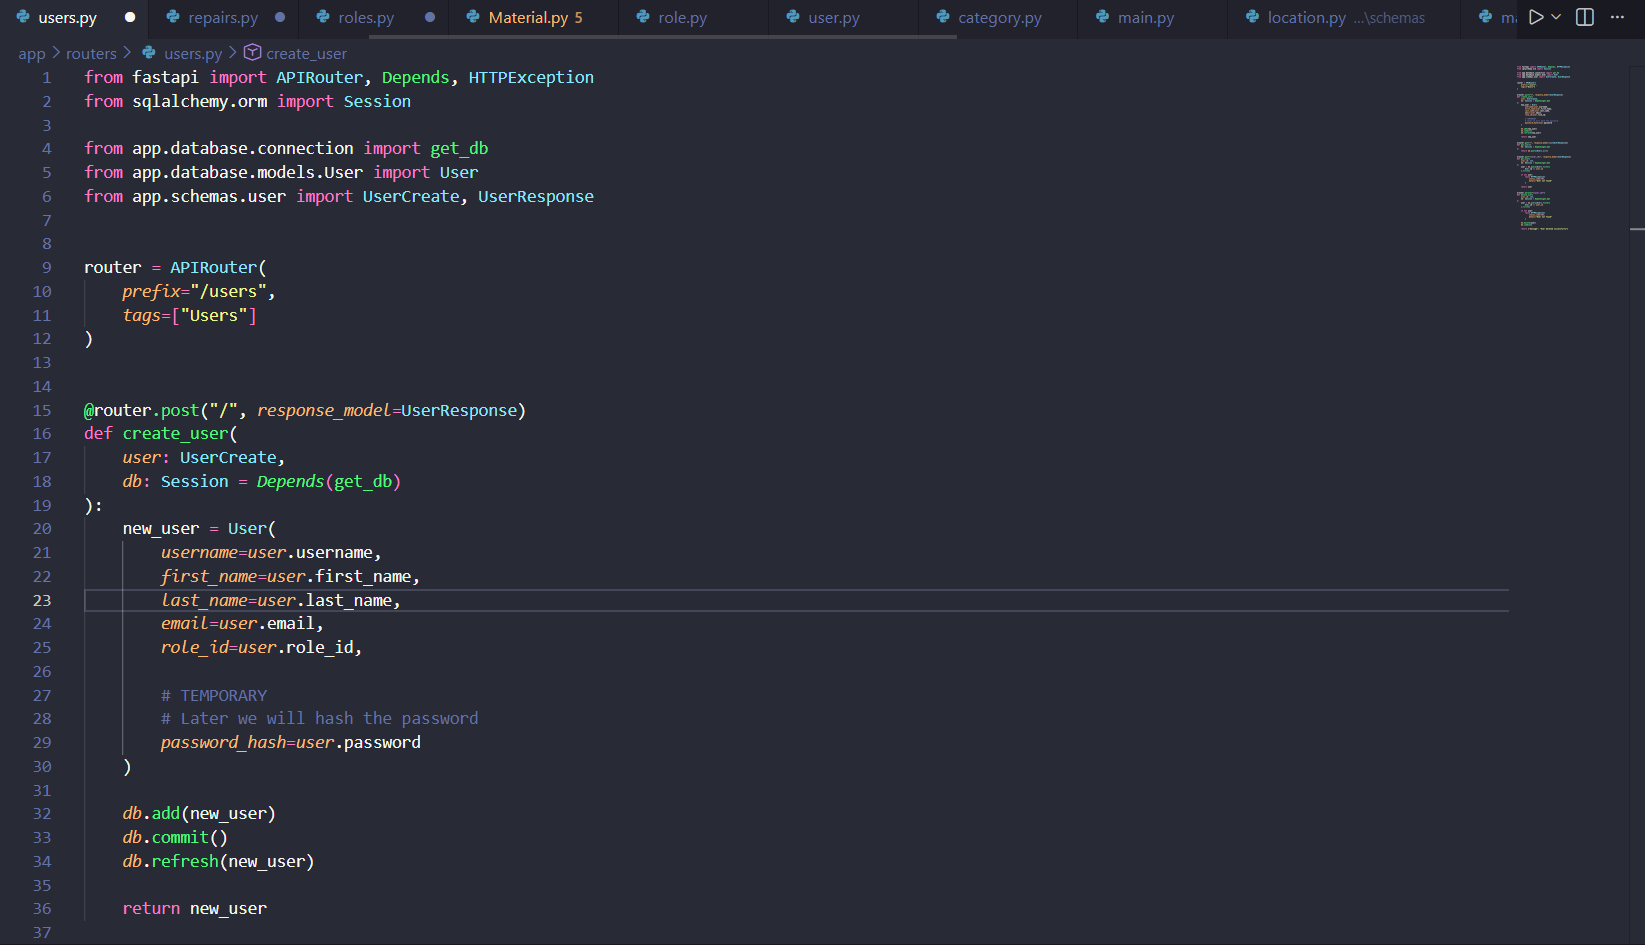
\includegraphics[width=0.8\textwidth]{screenshots/usersroute}
    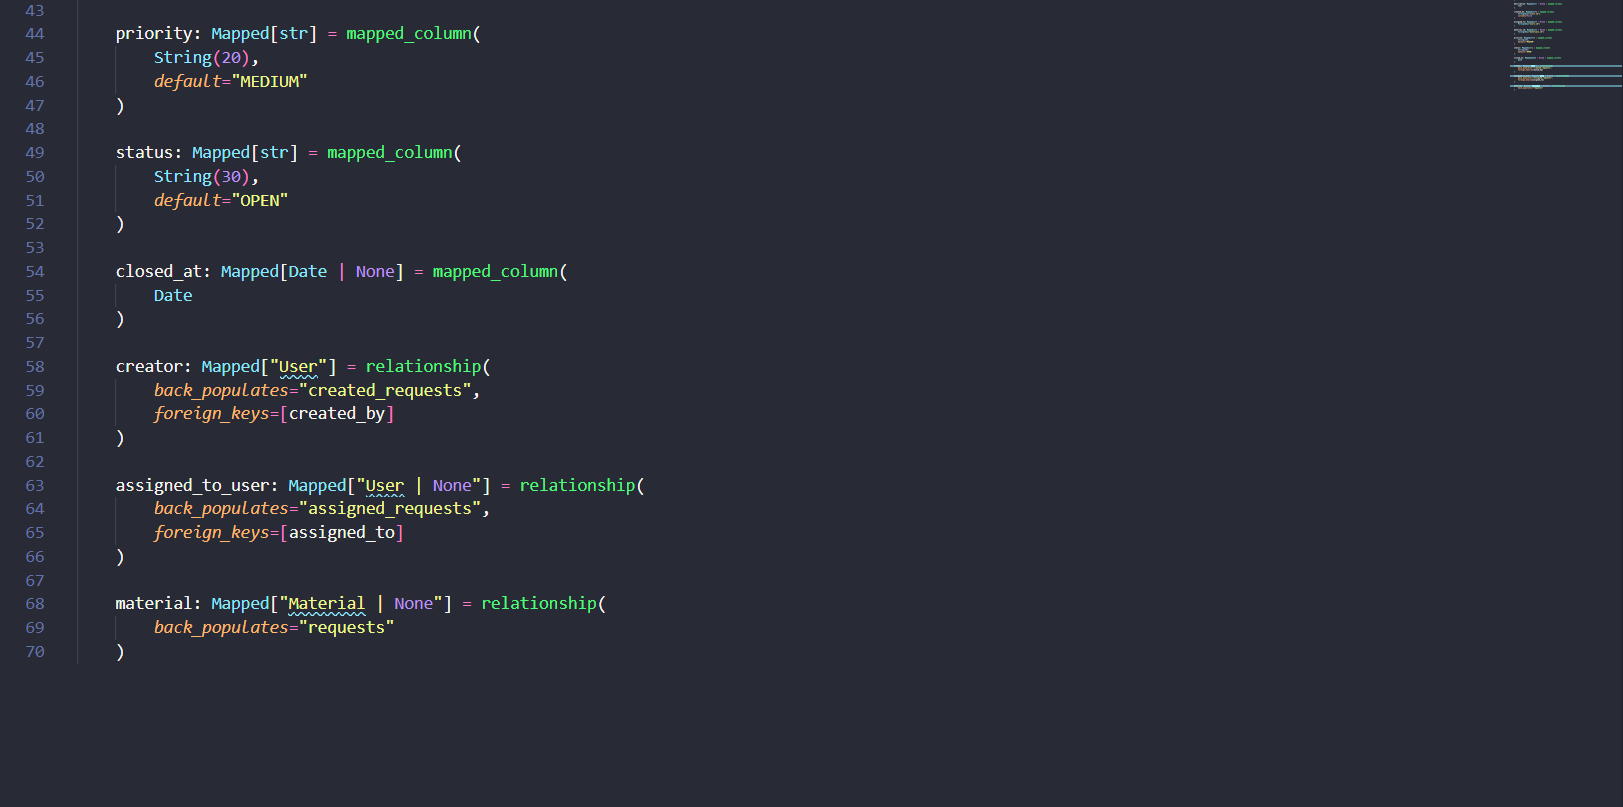
\includegraphics[width=0.8\textwidth]{screenshots/request2.png}
    \caption{Modèle Request}
\end{figure}

% =========================================================
% 12. SCHEMAS
% =========================================================




\chapter{Routers FastAPI}

Les endpoints sont séparés dans plusieurs fichiers afin de maintenir une
architecture claire.

\begin{lstlisting}
routers/
|
+-- roles.py
+-- users.py
+-- materials.py
+-- categories.py
+-- locations.py
+-- repairs.py
+-- requests.py
\end{lstlisting}

Cette organisation évite de placer toutes les routes dans le fichier
\texttt{main.py}.

\begin{figure}[H]
    \centering
    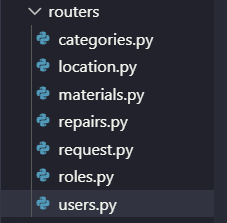
\includegraphics[width=0.8\textwidth]{screenshots/routers.png}
    \caption{Organisation des routers}
\end{figure}


% =========================================================
% 15. CRUD
% =========================================================

\section{Roles Route}
\begin{figure}[H]
    \centering
    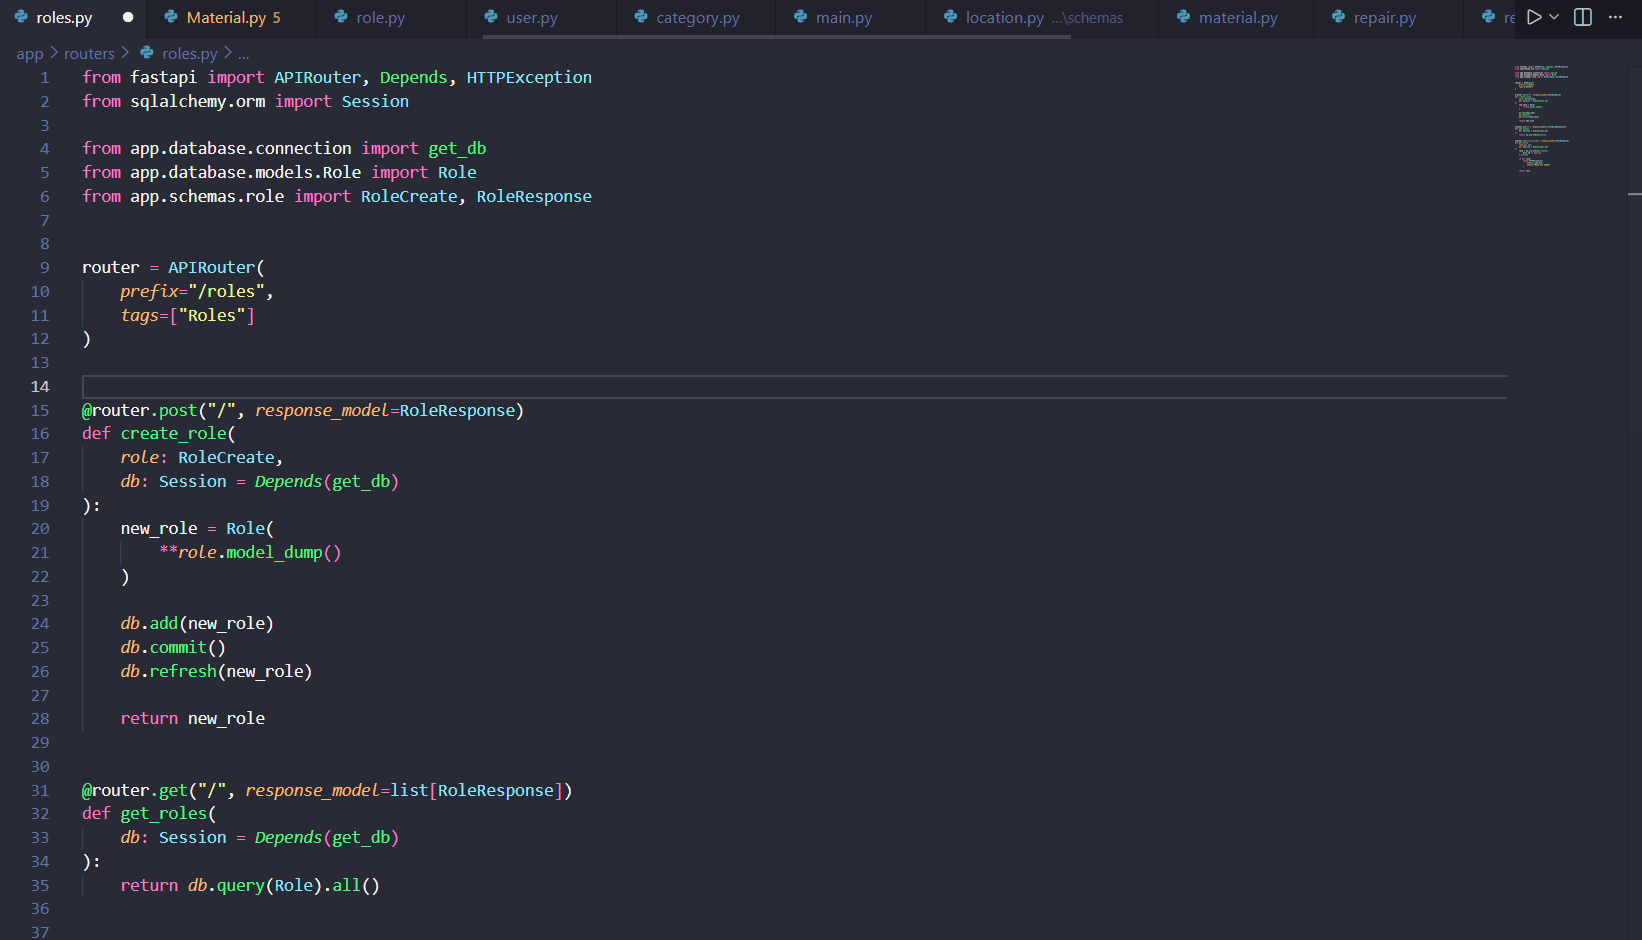
\includegraphics[width=0.8\textwidth]{screenshots/rolesroute.png}
    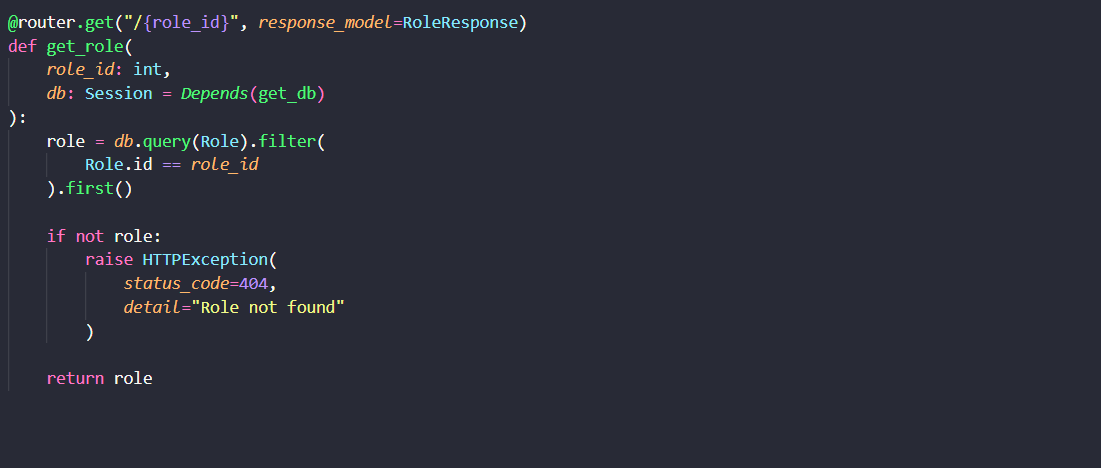
\includegraphics[width=0.8\textwidth]{screenshots/rolesroute1.png}
    \caption{Roles Route}
    \label{fig:getdb}
\end{figure}

\section{Users}
\begin{figure}[H]
    \centering
    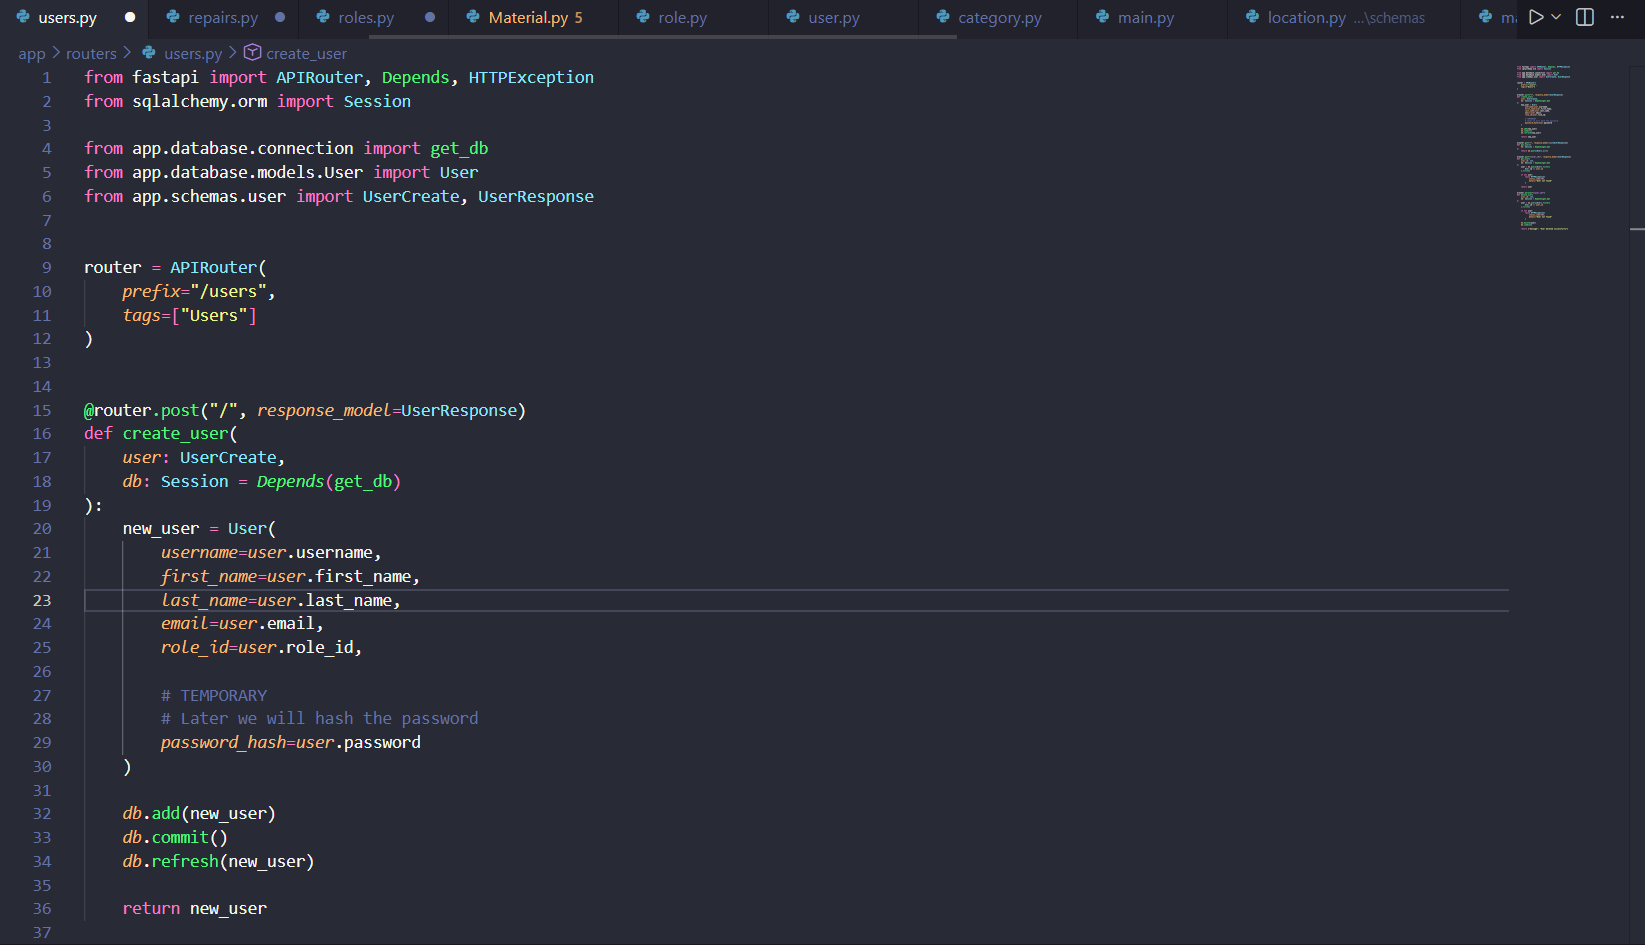
\includegraphics[width=0.8\textwidth]{screenshots/usersroute.png}
    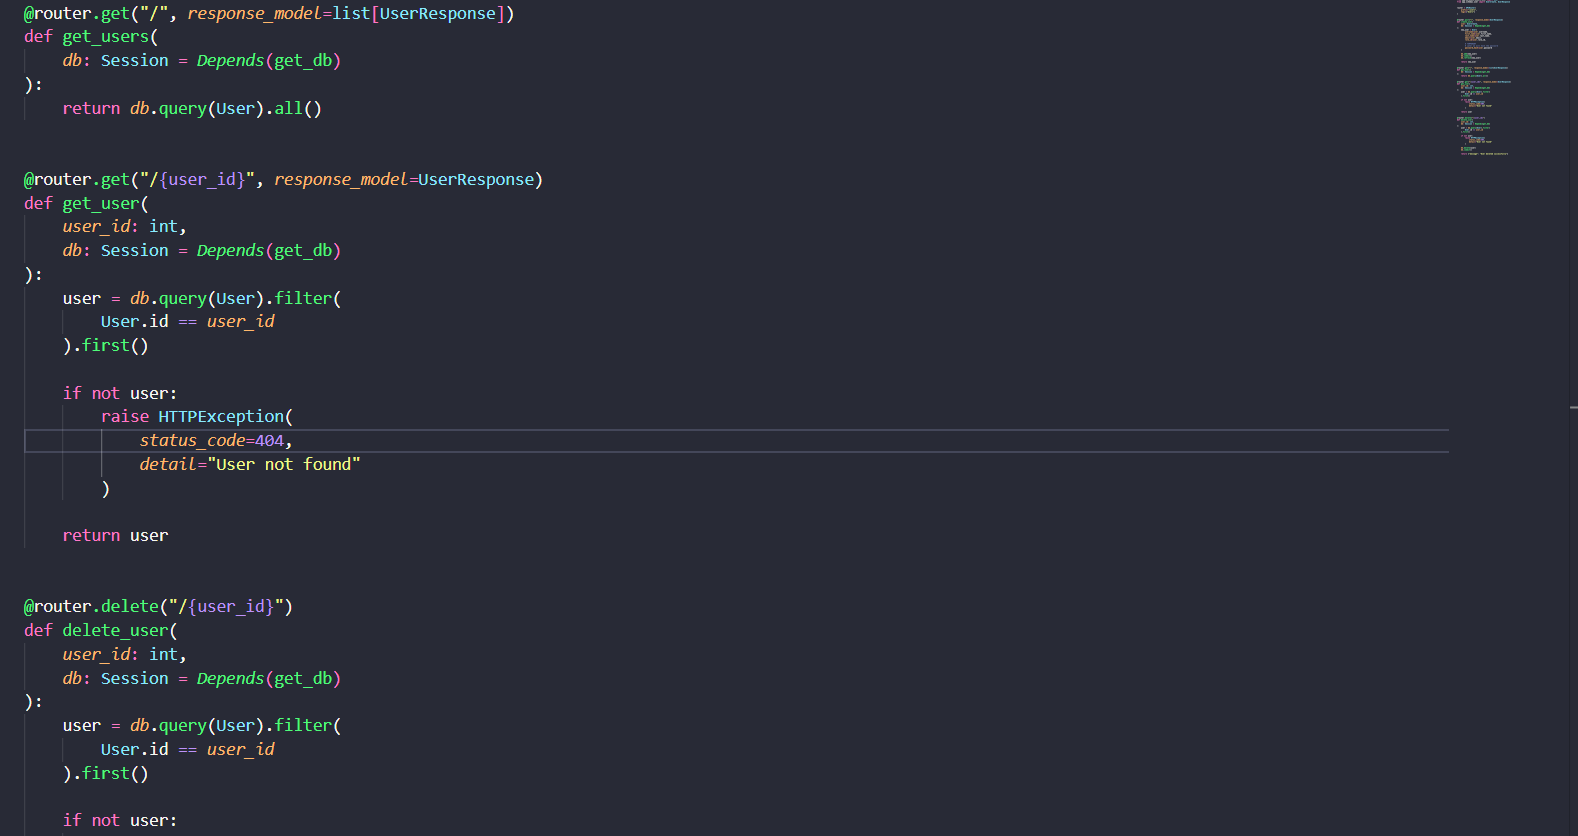
\includegraphics[width=0.8\textwidth]{screenshots/usersroute1.png}
    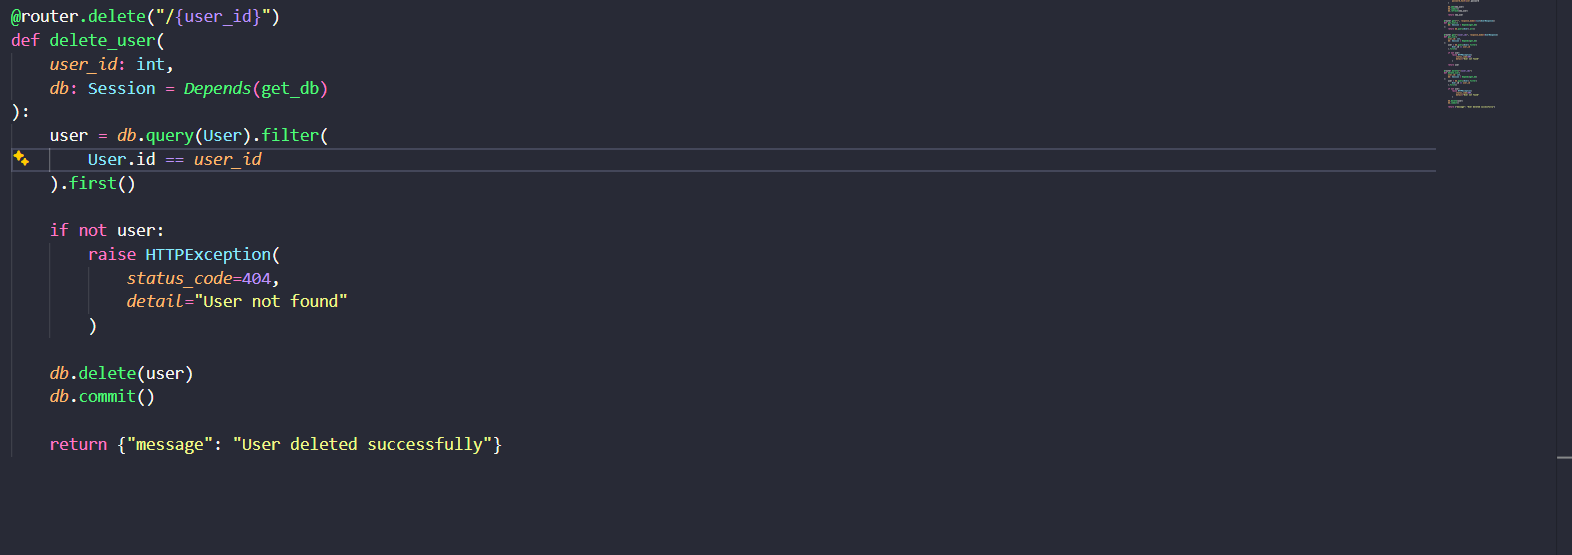
\includegraphics[width=0.8\textwidth]{screenshots/usersroute2.png}
    
    \caption{Users Route}
    \label{fig:getdb}
\end{figure}

\section{Materials route}
\begin{figure}[H]
    \centering
    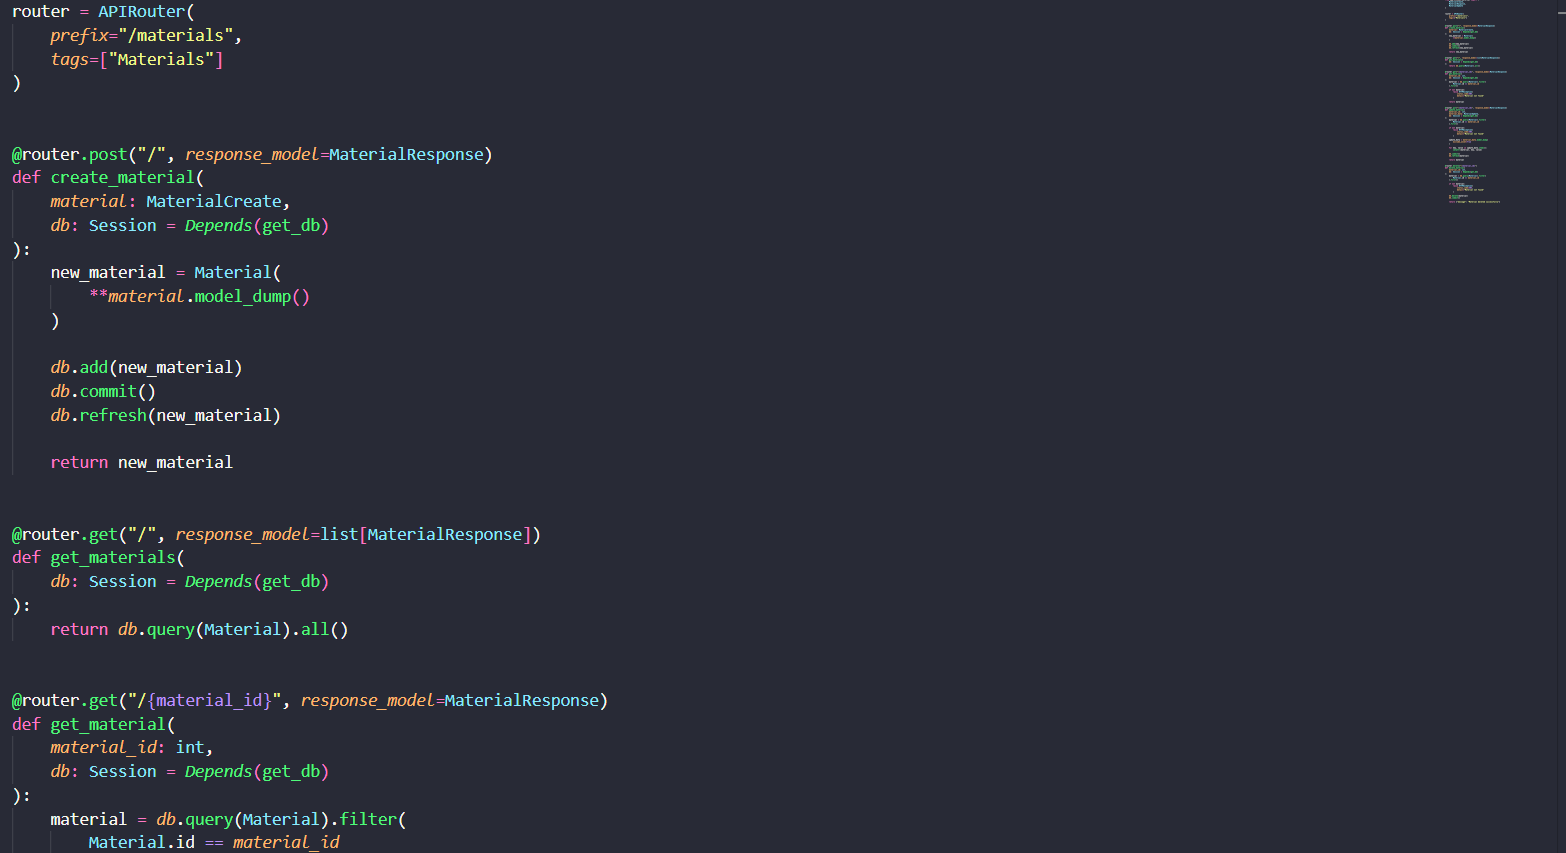
\includegraphics[width=0.8\textwidth]{screenshots/materialroute.png}
    \caption{Materials Route}
    \label{fig:getdb}
\end{figure}

\section{Categories}
\begin{figure}[H]
    \centering
    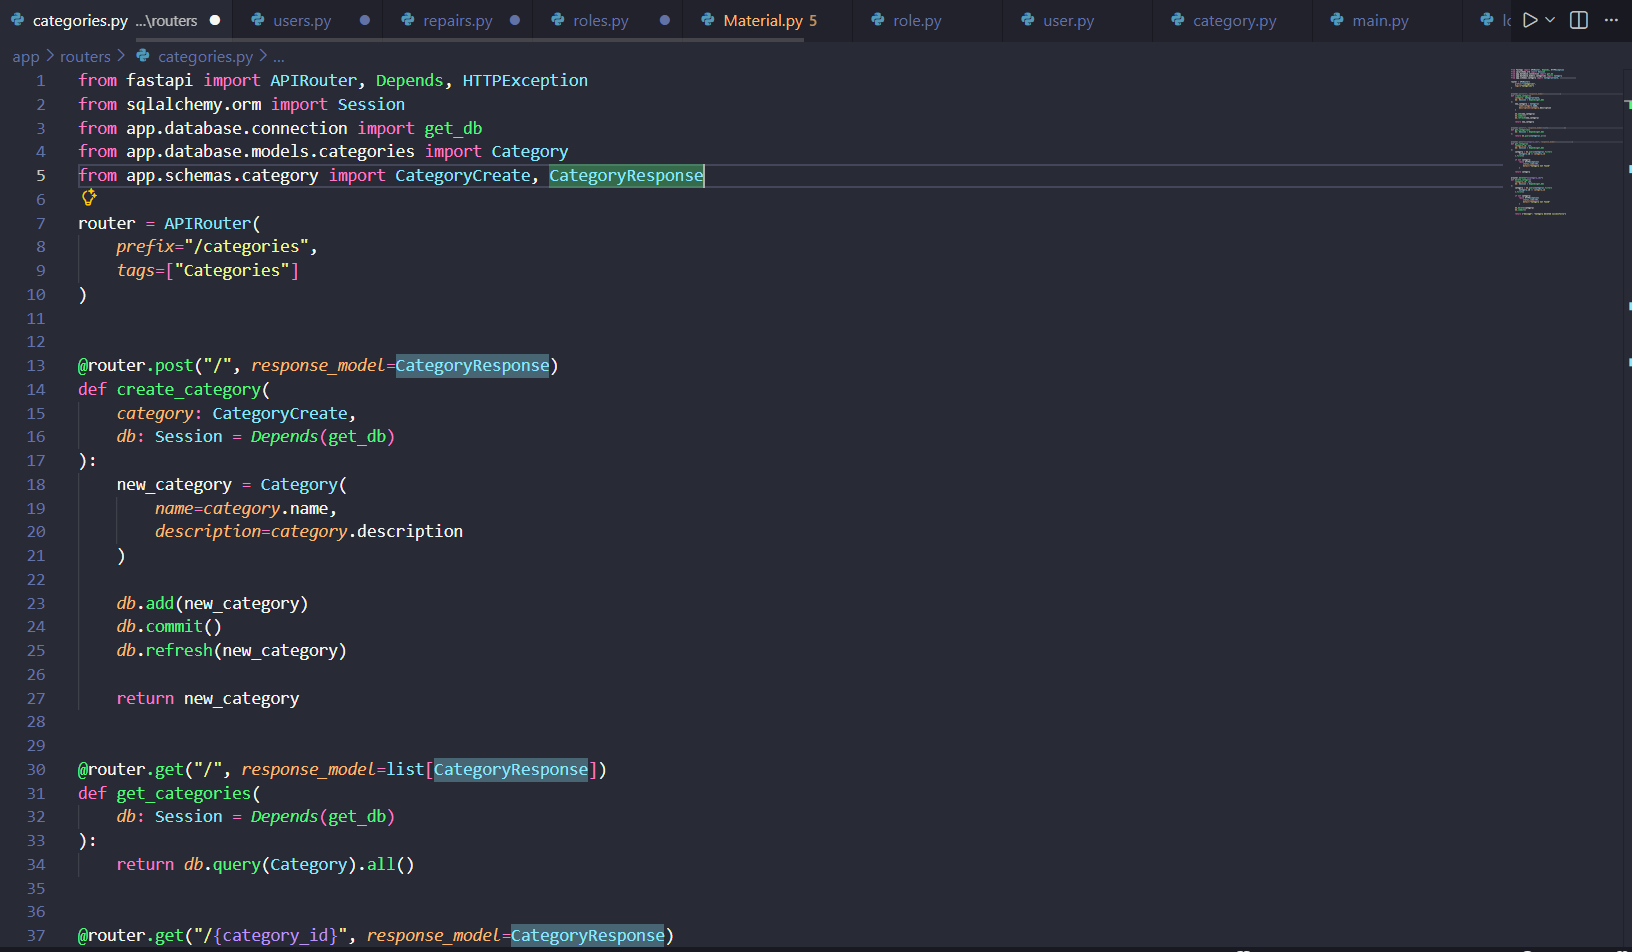
\includegraphics[width=0.8\textwidth]{screenshots/categoriesroute.png}
    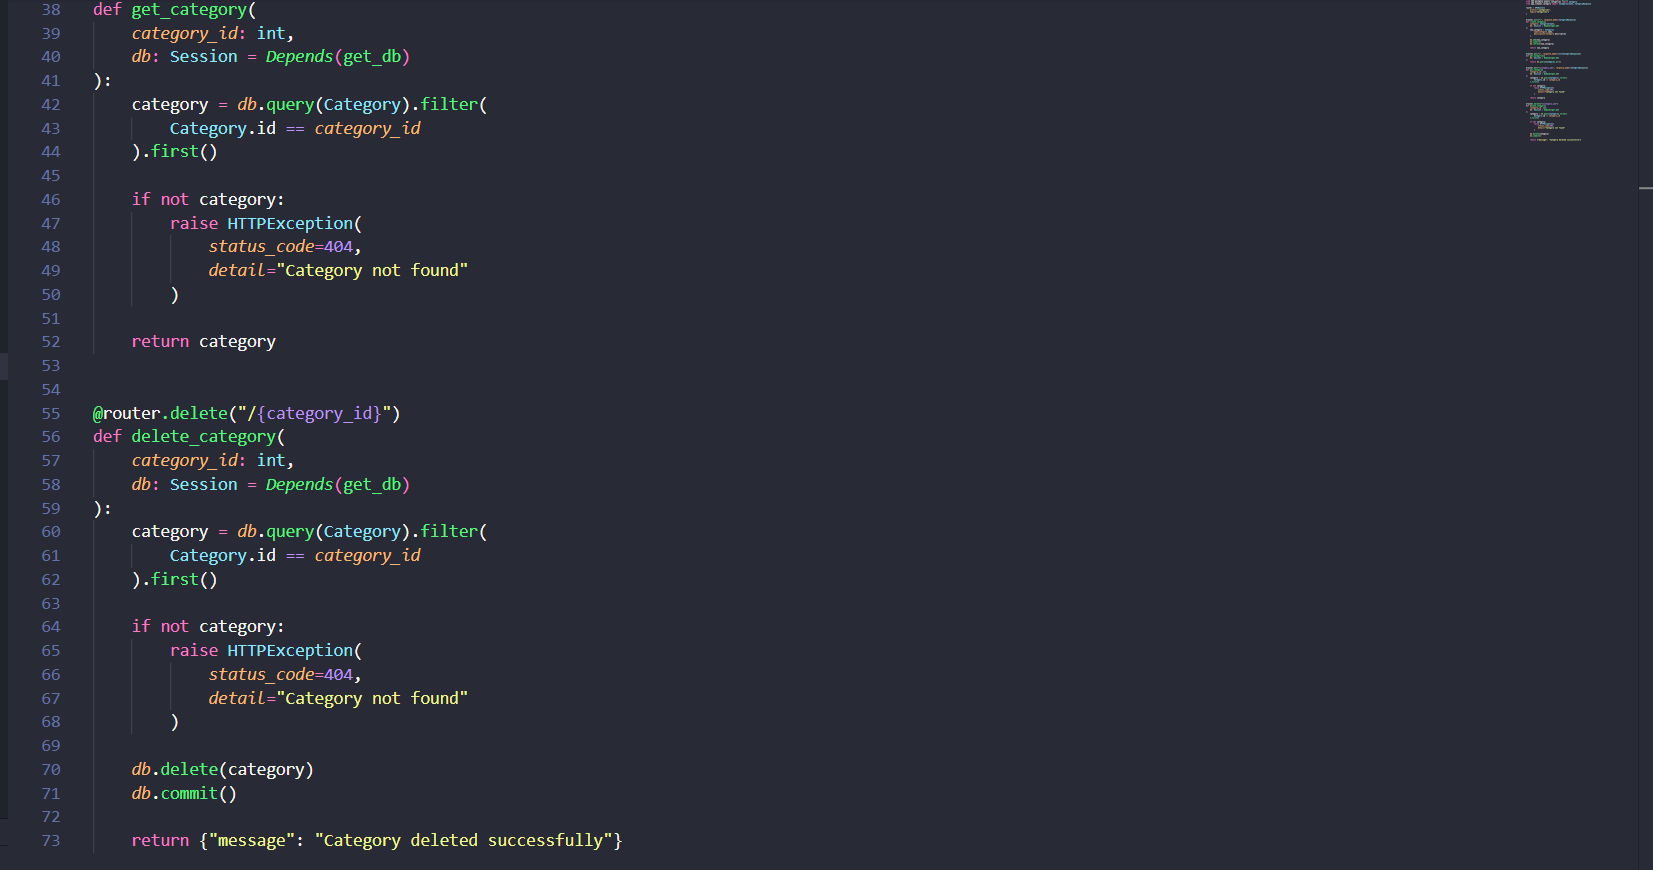
\includegraphics[width=0.8\textwidth]{screenshots/categories1.png}
    \caption{Roles Route}
    \label{fig:getdb}
\end{figure}
\section{Locations}
\begin{figure}[H]
    \centering
    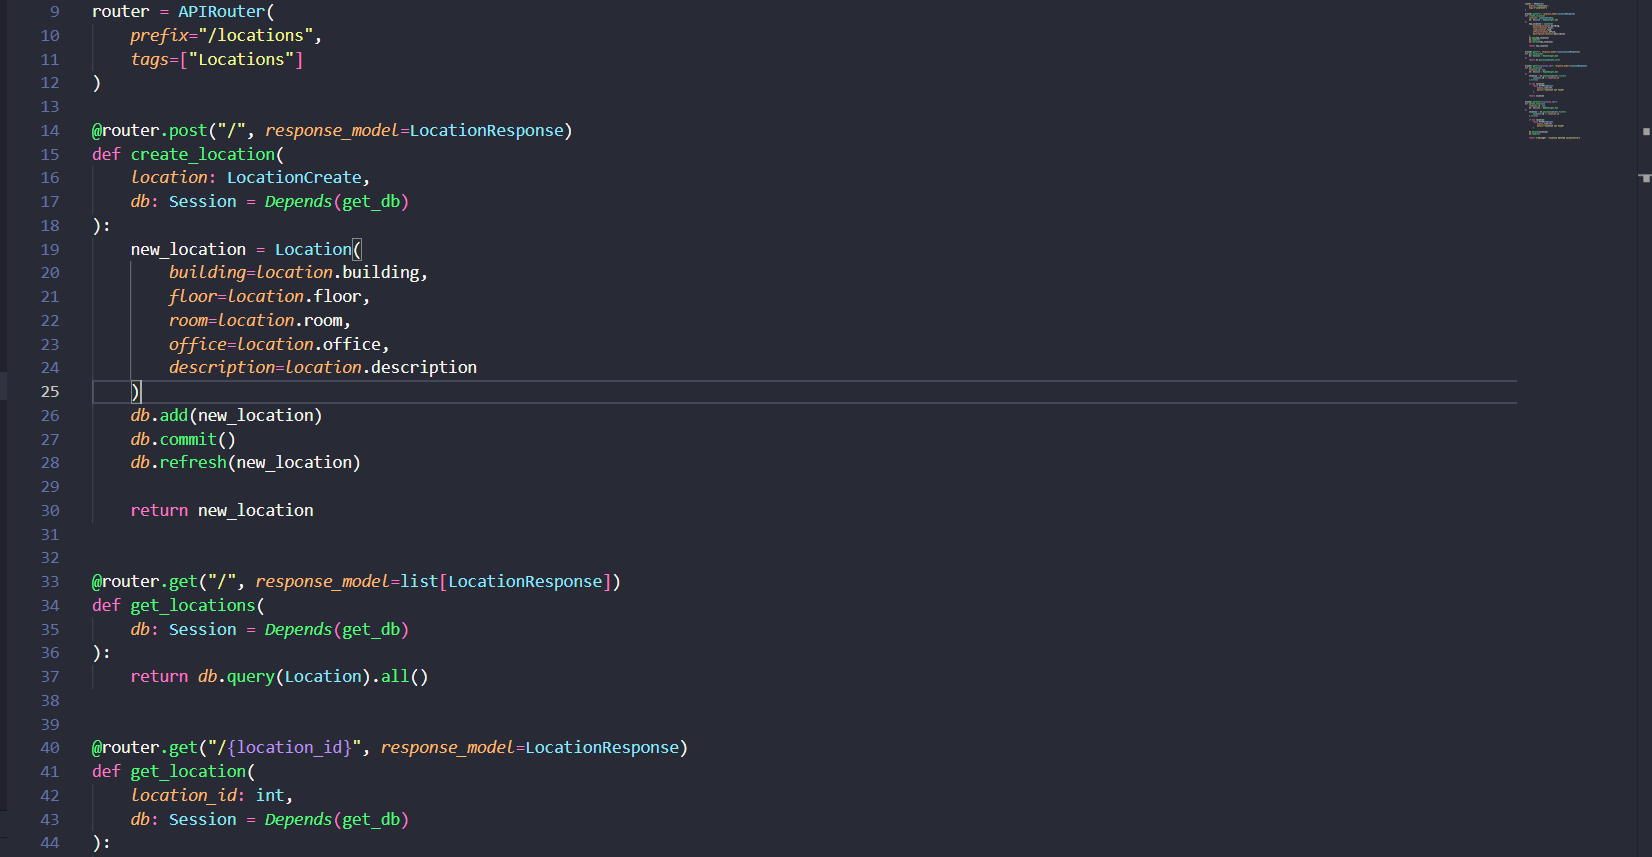
\includegraphics[width=0.8\textwidth]{screenshots/locationroute.png}
    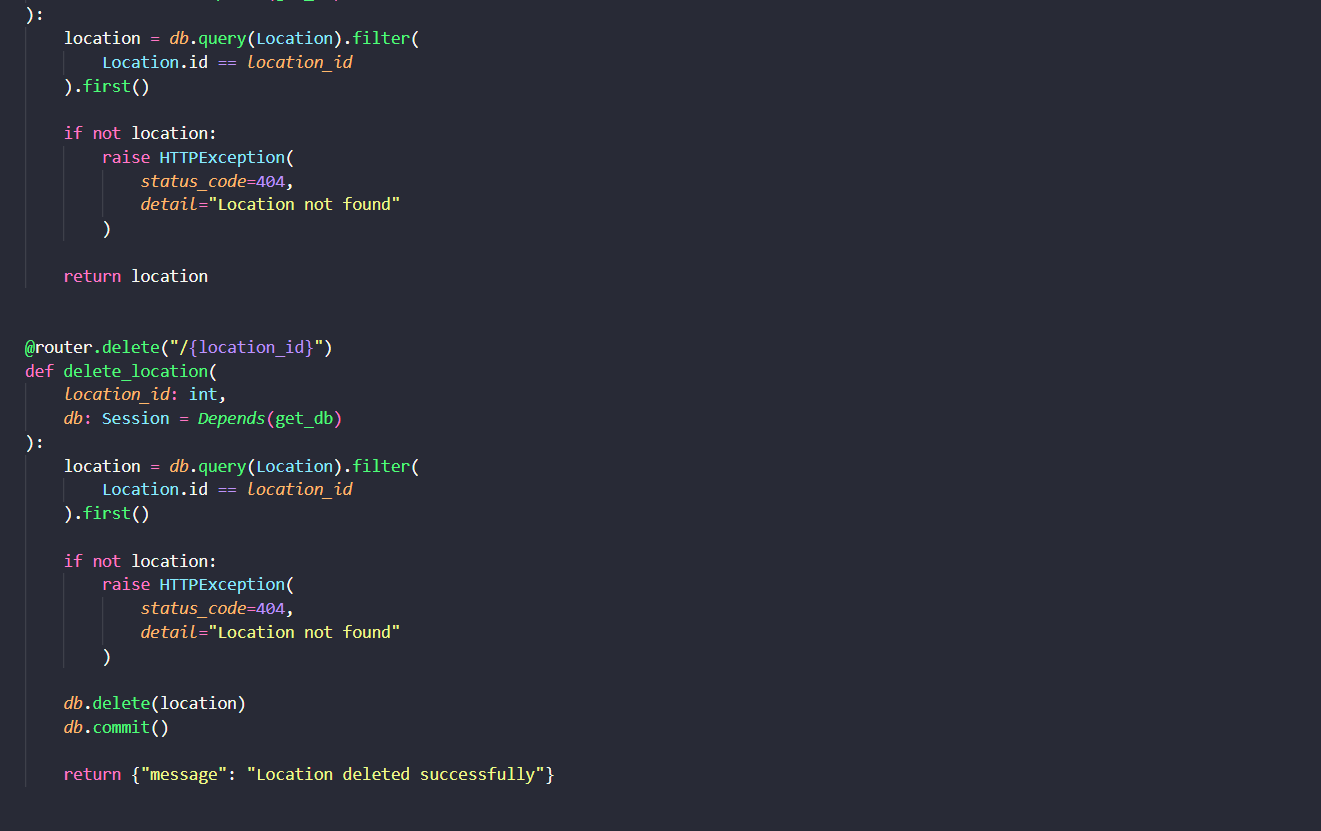
\includegraphics[width=0.8\textwidth]{screenshots/locationroute2.png}
    \caption{Roles Route}
    \label{fig:getdb}
\end{figure}

\section{Repairs}
\begin{figure}[H]
    \centering
    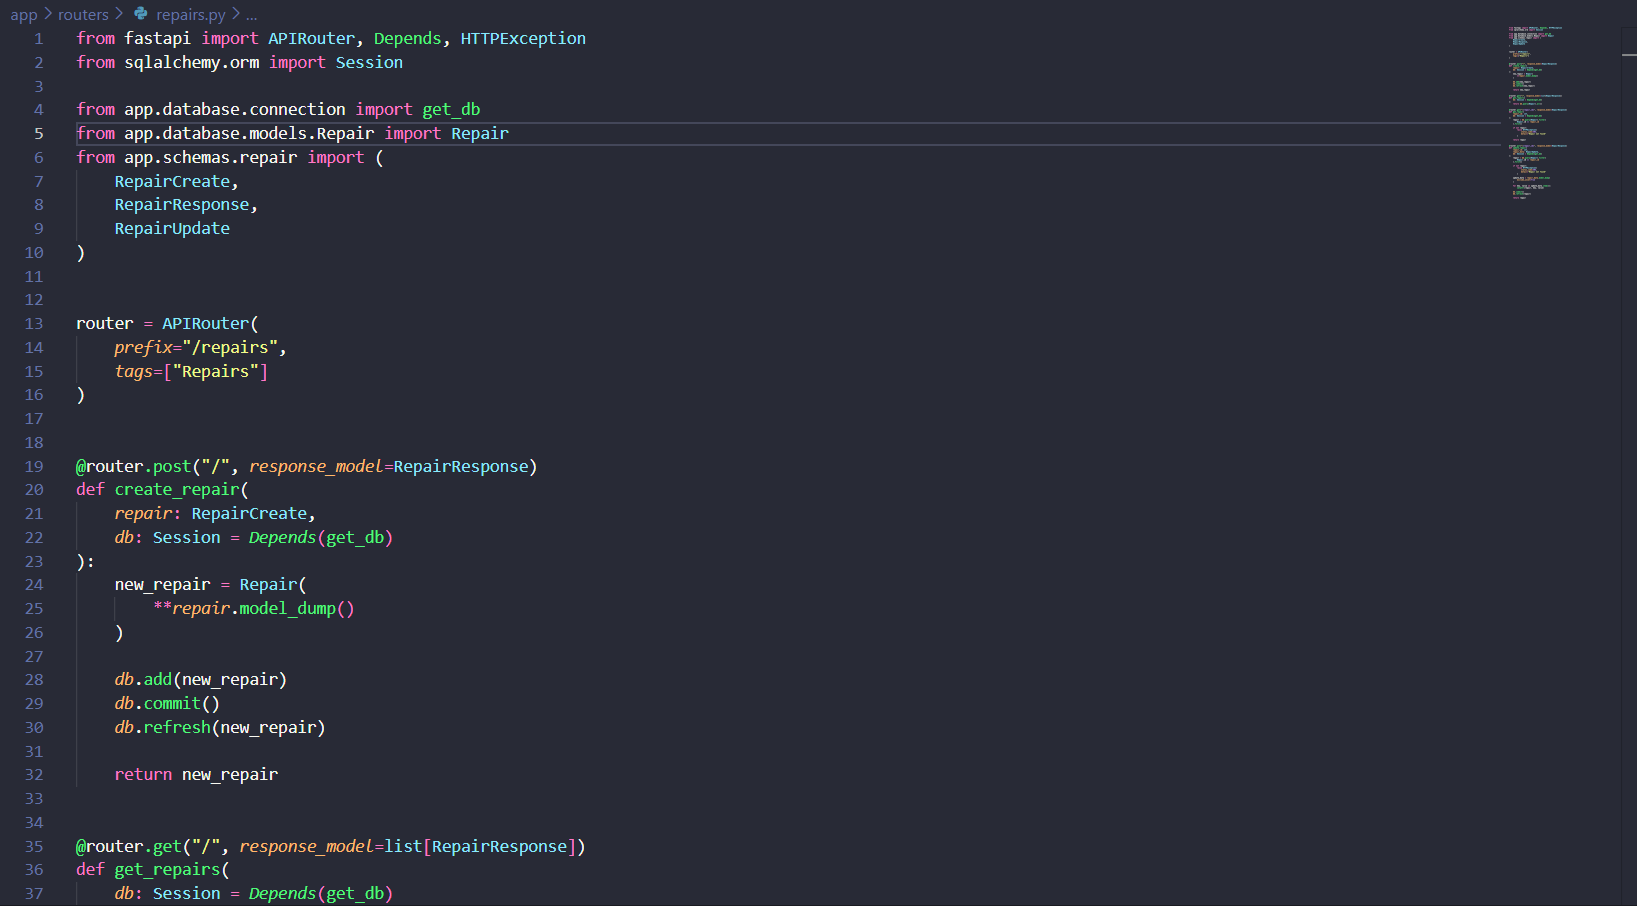
\includegraphics[width=0.8\textwidth]{screenshots/repairroute.png}
    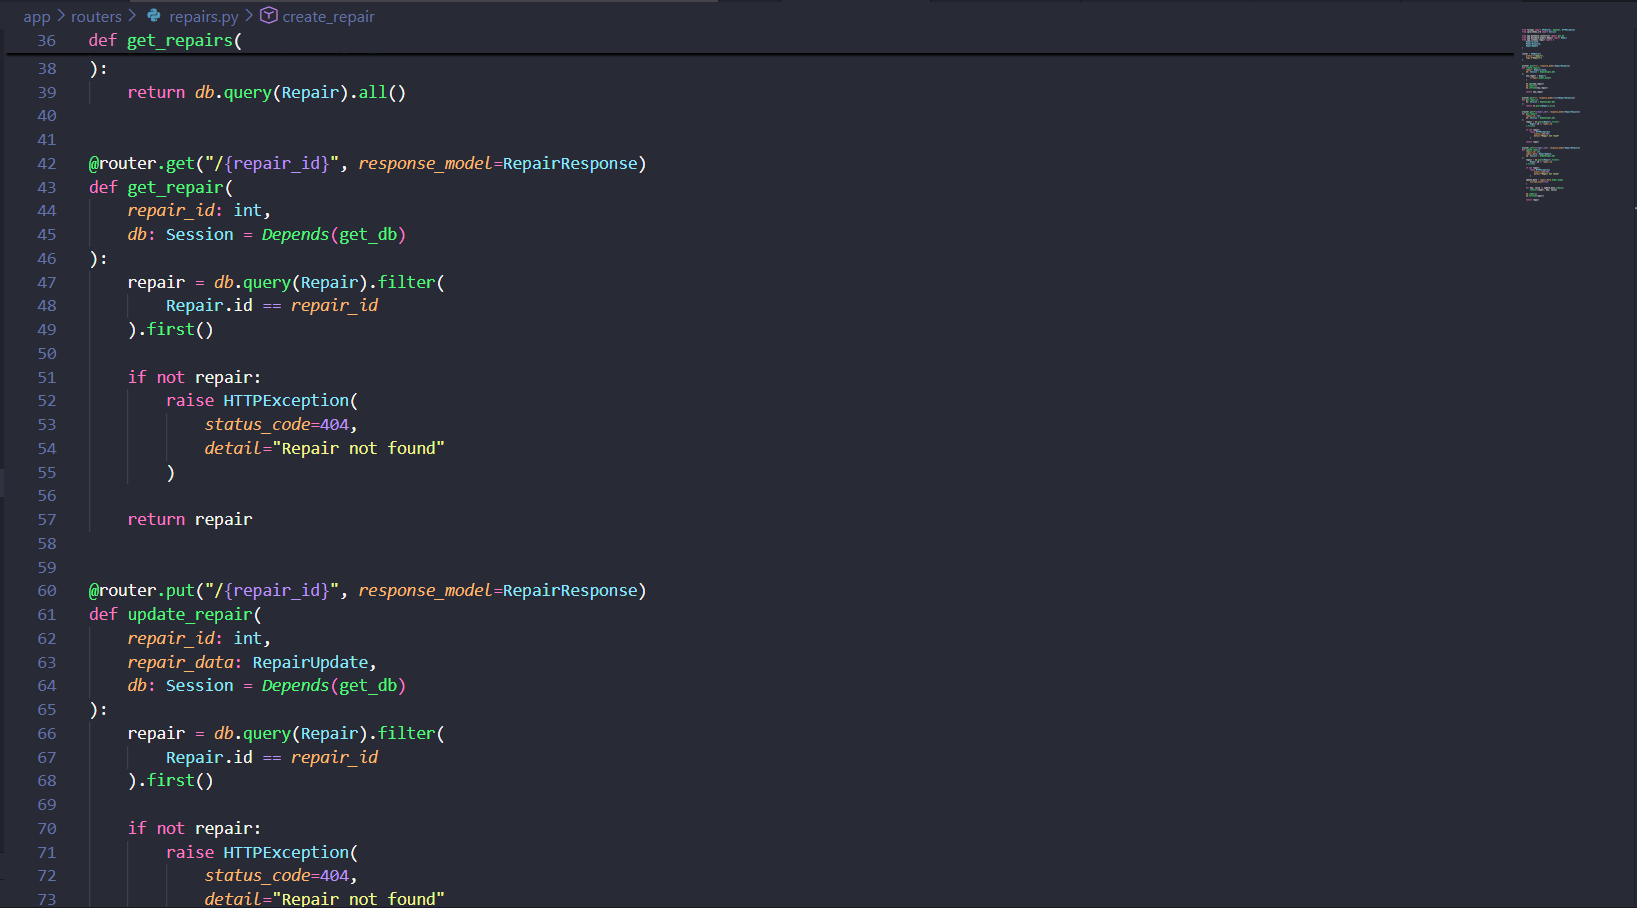
\includegraphics[width=0.8\textwidth]{screenshots/repairsroute1.png}
    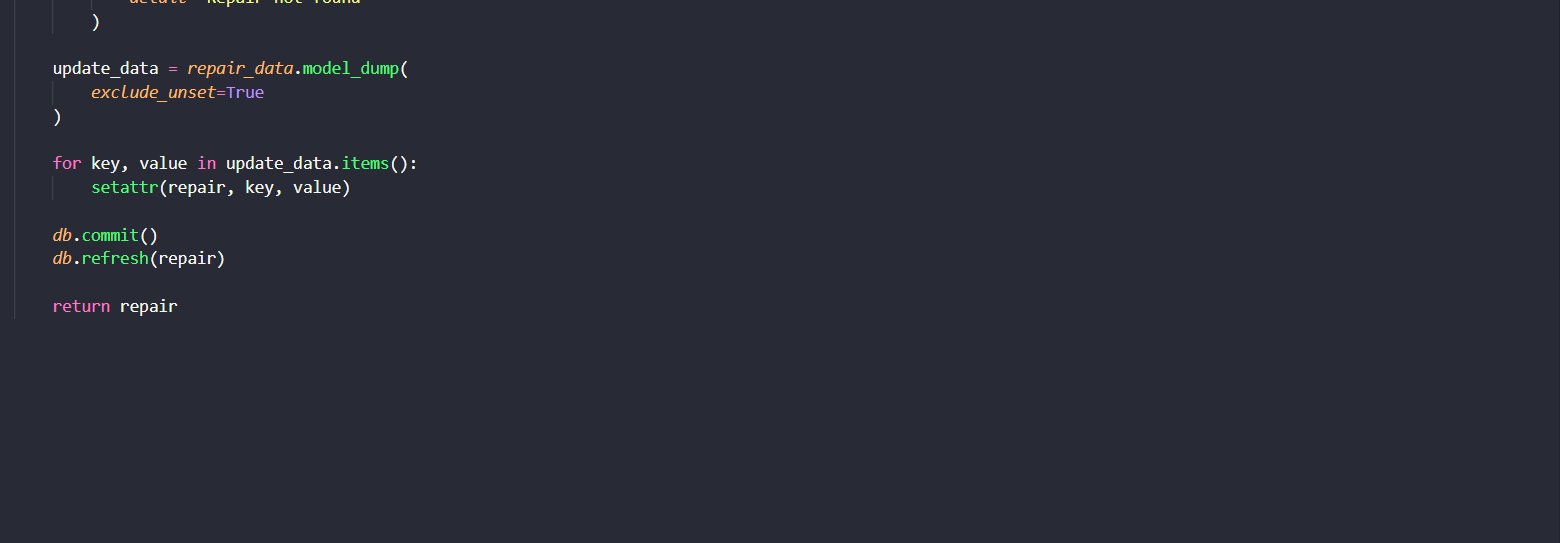
\includegraphics[width=0.8\textwidth]{screenshots/repairsroute2.png}
    \caption{Roles Route}
    \label{fig:getdb}
\end{figure}
\section{Requests}
\begin{figure}[H]
    \centering
    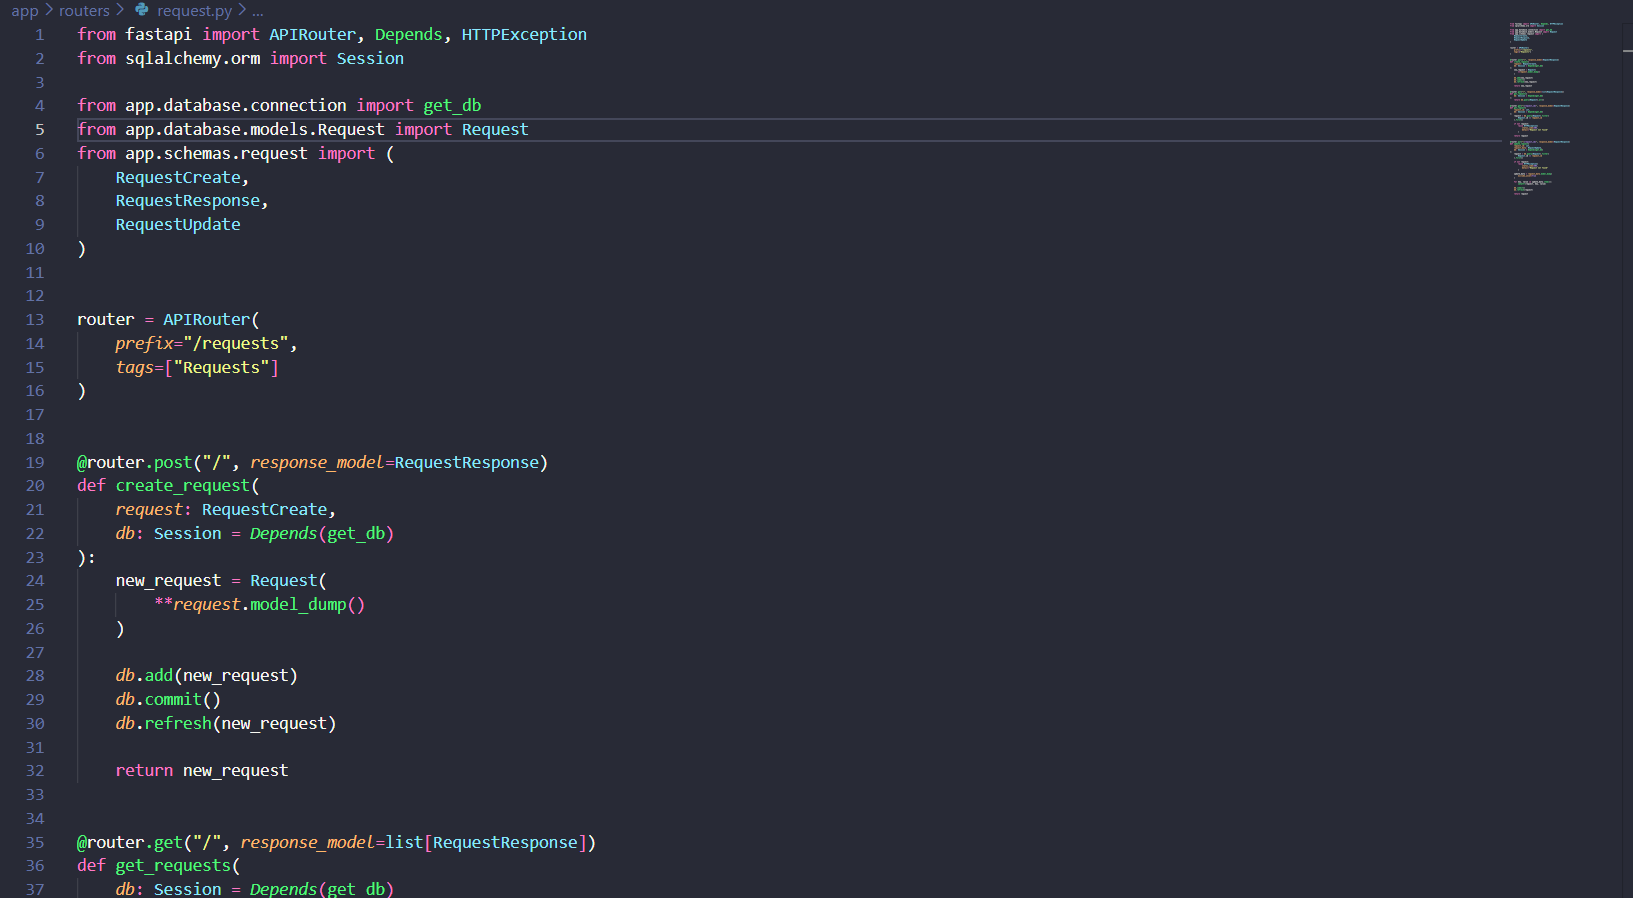
\includegraphics[width=0.8\textwidth]{screenshots/requestroute2.png}
    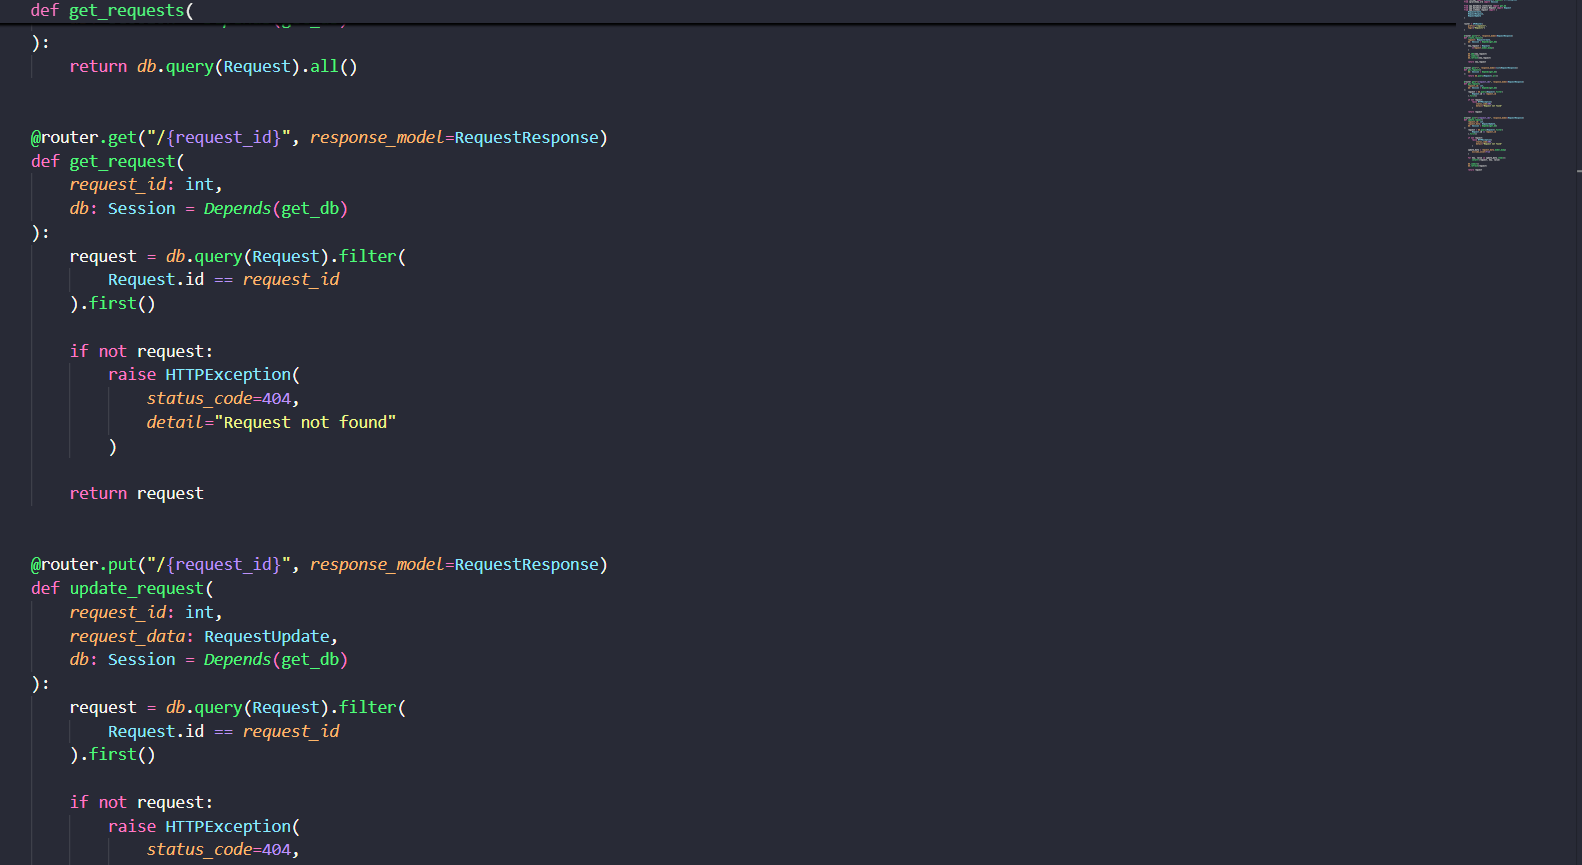
\includegraphics[width=0.8\textwidth]{screenshots/requestroute1.png}
    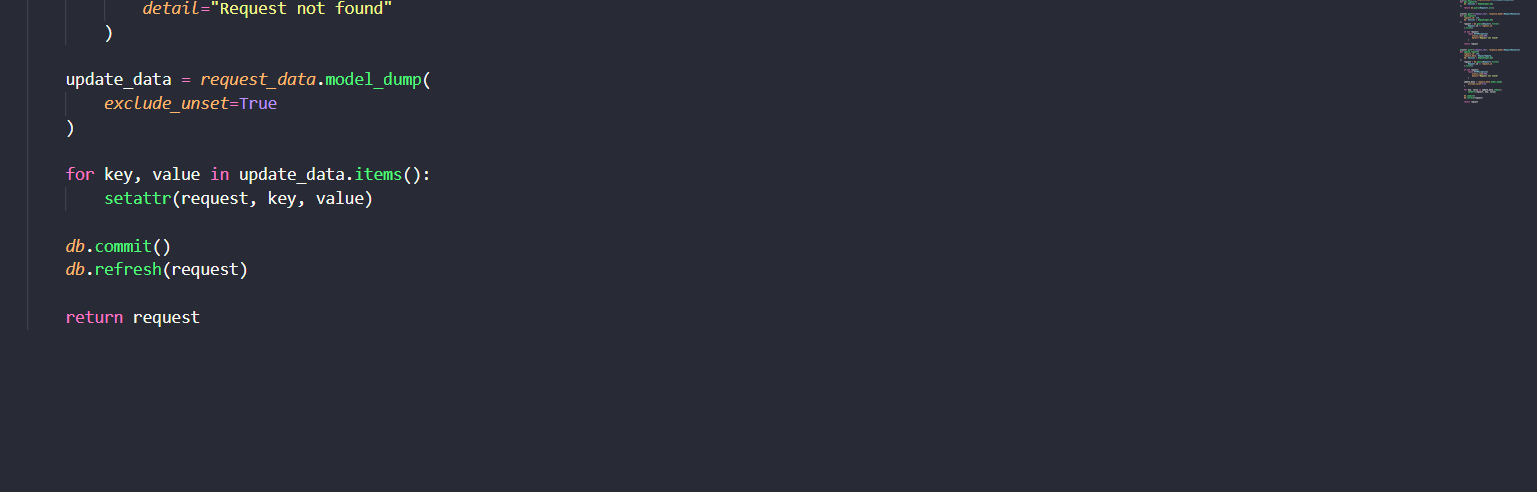
\includegraphics[width=0.8\textwidth]{screenshots/requestroute.png}
    \caption{Roles Route}
    \label{fig:getdb}
\end{figure}

\chapter{Point d'entrée de l'application}

Le fichier \texttt{main.py} constitue le point d'entrée de l'application
FastAPI.

L'application est créée avec :

\begin{lstlisting}[language=Python]
app = FastAPI(
    title="IT Park Management API"
)
\end{lstlisting}

Les différents routers sont ensuite enregistrés :

\begin{lstlisting}[language=Python]
app.include_router(materials.router)
app.include_router(users.router)
app.include_router(repairs.router)
app.include_router(requests.router)
\end{lstlisting}

Cette approche permet de garder le fichier \texttt{main.py} simple et
d'organiser la logique des endpoints dans les routers correspondants.

\begin{figure}[H]
    \centering
    \fbox{
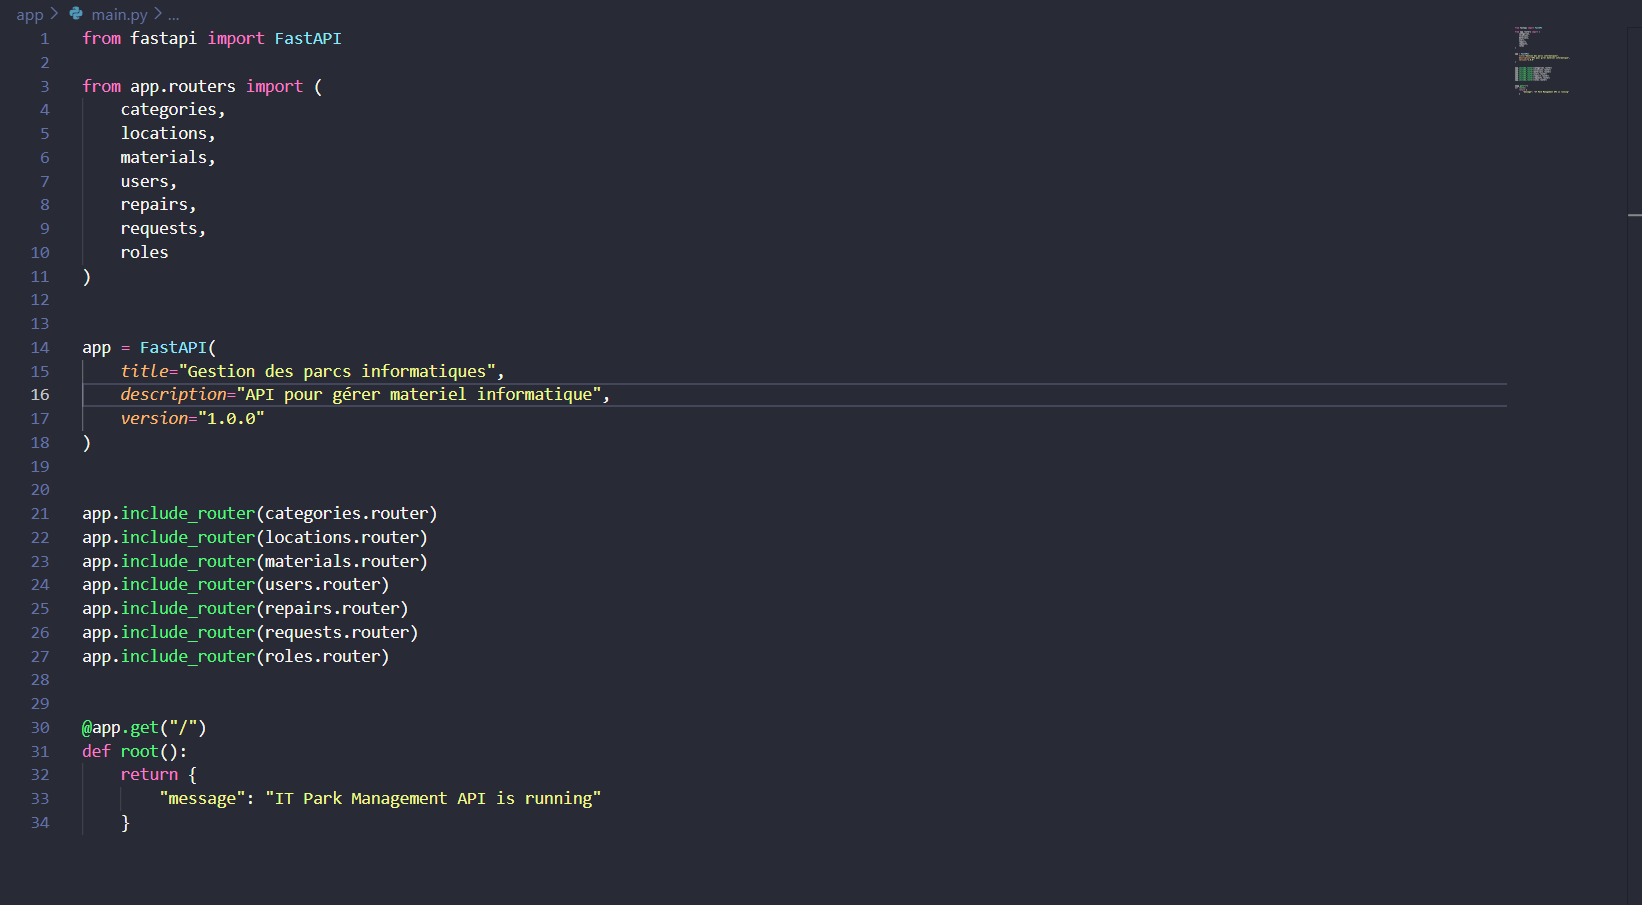
\includegraphics[width=0.8\textwidth]{screenshots/main.png}
    }
    \caption{Point d'entrée de l'application FastAPI}
\end{figure}

% =========================================================
% 21. SWAGGER
% =========================================================

\chapter{Architecture globale du backend}

Le fonctionnement général du backend peut être résumé comme suit :

\begin{center}

\begin{tabular}{c}
Frontend \\[0.2cm]
$\downarrow$ \\[0.2cm]
FastAPI \\[0.2cm]
$\downarrow$ \\[0.2cm]
Routers \\[0.2cm]
$\downarrow$ \\[0.2cm]
Schémas Pydantic \\[0.2cm]
$\downarrow$ \\[0.2cm]
Modèles SQLAlchemy \\[0.2cm]
$\downarrow$ \\[0.2cm]
PostgreSQL
\end{tabular}

\end{center}

Cette architecture permet de séparer clairement les différentes
responsabilités de l'application.


% =========================================================
% 23. ETAT
% =========================================================

\chapter{Authentification et sécurité}

\section{Objectif}

L'authentification permet de vérifier l'identité de l'utilisateur avant
de lui donner accès aux ressources protégées.

Le système utilise :

\begin{itemize}
    \item un mot de passe utilisateur ;
    \item un mécanisme de hachage sécurisé ;
    \item JSON Web Token (JWT) ;
    \item une dépendance \texttt{get\_current\_user} ;
    \item une dépendance \texttt{require\_role} pour l'autorisation.
\end{itemize}

\section{Hachage du mot de passe}

Le mot de passe ne doit jamais être stocké directement dans la base
de données.

Lors de la création d'un utilisateur :

\begin{verbatim}
Mot de passe
      |
      v
Fonction de hachage
      |
      v
password_hash
      |
      v
PostgreSQL
\end{verbatim}

La base contient donc le hash du mot de passe et non le mot de passe
en clair.
\begin{figure}[H]
    \centering
    \fbox{
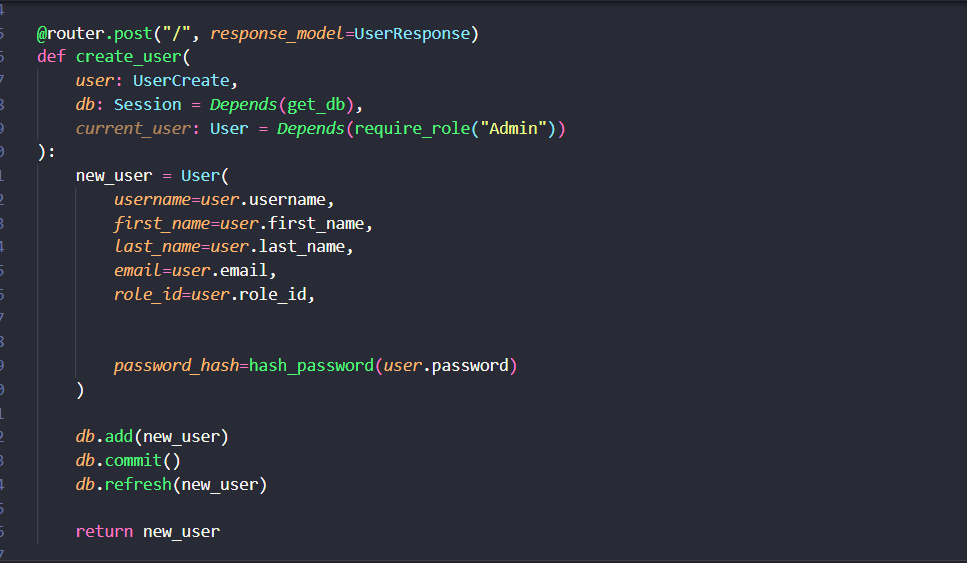
\includegraphics[width=0.8\textwidth]{screenshots/hashage password.png}
    }
    \caption{Hachage du mot de passe avant son stockage}
\end{figure}

\section{Connexion}

L'utilisateur fournit son identifiant et son mot de passe à
l'endpoint de connexion :

\begin{verbatim}
POST /auth/login
\end{verbatim}

Le backend vérifie :

\begin{enumerate}
    \item que l'utilisateur existe ;
    \item que le mot de passe correspond au hash stocké ;
    \item que le compte est autorisé à se connecter.
\end{enumerate}

Si les informations sont correctes, un JWT est généré.

\section{JWT}

Le JSON Web Token représente une preuve d'authentification temporaire.

Le fonctionnement général est :

\begin{verbatim}
username + password
        |
        v
   Vérification
        |
        v
      JWT
        |
        v
Authorization: Bearer <token>
\end{verbatim}

\begin{figure}[H]
    \centering
    \fbox{
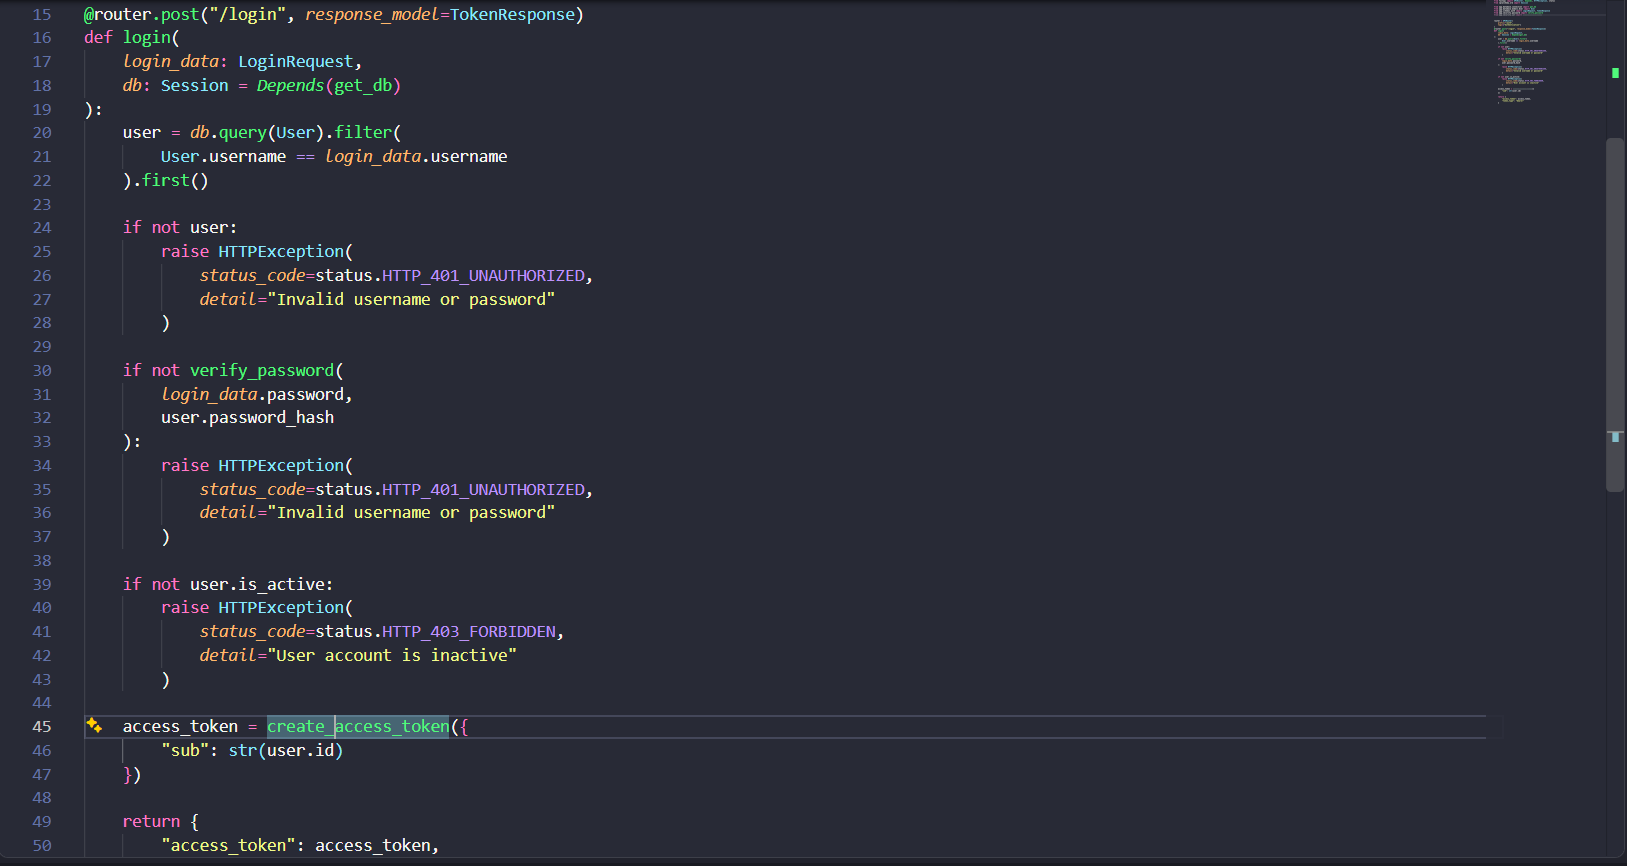
\includegraphics[width=0.8\textwidth]{screenshots/create access token.png}
    }
    \caption{Authentification et génération du JWT}
\end{figure}


\section{get\_current\_user}

La fonction \texttt{get\_current\_user()} permet de récupérer
l'utilisateur correspondant au JWT envoyé avec la requête.

Elle est utilisée avec FastAPI :

\begin{lstlisting}
current_user: User = Depends(
    get_current_user
)
\end{lstlisting}

Dans ce cas, \texttt{User} représente le modèle SQLAlchemy.

La fonction permet donc de récupérer l'utilisateur depuis la base de
données.

Le processus est :

\begin{verbatim}
Authorization Header
        |
        v
Bearer JWT
        |
        v
Validation du token
        |
        v
Récupération de l'identifiant
        |
        v
Recherche dans PostgreSQL
        |
        v
User SQLAlchemy
\end{verbatim}

\section{Protection d'un endpoint}

Lorsqu'un endpoint est accessible à tous les utilisateurs
authentifiés :

\begin{lstlisting}
@router.get("/")
def get_materials(
    db: Session = Depends(get_db),
    current_user: User = Depends(
        get_current_user
    )
):
    ...
\end{lstlisting}

L'utilisateur doit donc posséder un token valide.

\begin{figure}[H]
    \centering
    \fbox{
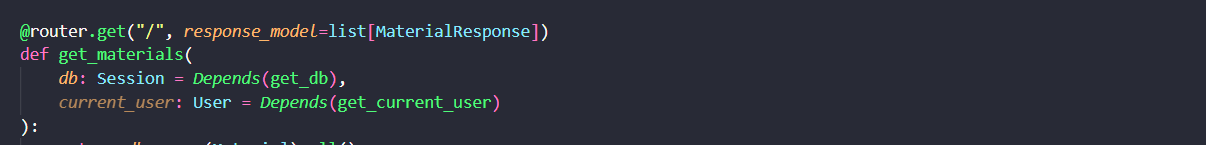
\includegraphics[width=0.8\textwidth]{screenshots/get current user.png}
    }
    \caption{Utilisation de get current user dans un endpoint protégé}
\end{figure}

% {12_get_current_user.png}
% {Utilisation de get_current_user dans un endpoint protégé}
% {fig:get-current-user}

% ============================================================
% AUTORISATION
% ============================================================

\chapter{Autorisation et gestion des rôles}

\section{Différence entre authentification et autorisation}

L'authentification répond à la question :

\begin{center}
\textit{« Qui est l'utilisateur ? »}
\end{center}

L'autorisation répond à la question :

\begin{center}
\textit{« A-t-il le droit d'effectuer cette opération ? »}
\end{center}

\section{require\_role}

La fonction \texttt{require\_role()} permet de limiter l'accès à un
endpoint selon le rôle de l'utilisateur.

Par exemple :

\begin{lstlisting}
current_user: User = Depends(
    require_role("Admin")
)
\end{lstlisting}

Dans ce cas, \texttt{require\_role()} appelle déjà
\texttt{get\_current\_user()}.

Il n'est donc pas nécessaire d'utiliser les deux dépendances
séparément sur le même endpoint.

\section{Fonctionnement}

\begin{verbatim}
Requête
   |
   v
JWT valide ?
   |
   +---- Non ----> 401 Unauthorized
   |
  Oui
   |
   v
Récupérer User
   |
   v
Vérifier le rôle
   |
   +---- Rôle incorrect ----> 403 Forbidden
   |
  Correct
   |
   v
Autoriser l'accès
\end{verbatim}

\backendimage
{13_require_role.png}
{Contrôle d'accès selon le rôle de l'utilisateur}
{fig:require-role}

\section{Exemple}

Un endpoint réservé à l'administrateur peut être protégé ainsi :

\begin{lstlisting}
@router.delete("/{material_id}")
def delete_material(
    material_id: int,
    db: Session = Depends(get_db),
    current_user: User = Depends(
        require_role("Admin")
    )
):
    ...
\end{lstlisting}

Un utilisateur possédant un rôle différent obtient une réponse
\texttt{403 Forbidden}.

% ============================================================
% POSTMAN
% ============================================================

\chapter{Tests de l'API avec Postman}

\section{Objectif des tests}

Après l'implémentation du backend, plusieurs scénarios ont été
exécutés avec Postman afin de vérifier le comportement de l'API.

Les tests permettent notamment de vérifier :

\begin{itemize}
    \item la connexion à la base de données ;
    \item la création des rôles ;
    \item la création des utilisateurs ;
    \item le hachage des mots de passe ;
    \item la connexion utilisateur ;
    \item la génération du JWT ;
    \item l'accès aux endpoints protégés ;
    \item le refus d'un token invalide ;
    \item la gestion des permissions ;
    \item les opérations CRUD ;
    \item la gestion des réparations ;
    \item la gestion des demandes ;
    \item le comportement des utilisateurs inactifs.
\end{itemize}

\section{Test de création d'un rôle}

Requête :

\begin{verbatim}
POST /roles/
\end{verbatim}

Exemple :

\begin{lstlisting}
{
    "name": "Admin",
    "description": "System administrator"
}
\end{lstlisting}

Résultat attendu :

\begin{verbatim}
201 Created
\end{verbatim}
\begin{figure}[H]
    \centering
    \fbox{

\includegraphics[width=0.8\textwidth]{create role.png}
    }
    \caption{Création d'un rôle avec Postman}
\end{figure}


% \backendimage
% {14_postman_create_role.png}
% {Création d'un rôle avec Postman}
% {fig:postman-create-role}

\section{Test de création d'un utilisateur}

Exemple :

\begin{lstlisting}
{
    "username": "admin",
    "first_name": "System",
    "last_name": "Administrator",
    "email": "admin@example.com",
    "password": "Admin123!",
    "role_id": 1
}
\end{lstlisting}

Le mot de passe est haché avant d'être stocké.

\begin{figure}[H]
    \centering
    \fbox{

\includegraphics[width=0.8\textwidth]{creating user.png}
    }
    \caption{Création d'un utilisateur avec Postman}
\end{figure}

% \backendimage
% {15_postman_create_user.png}
% {Création d'un utilisateur avec Postman}
% {fig:postman-create-user}

\section{Test de connexion}

Requête :

\begin{verbatim}
POST /auth/login
\end{verbatim}

Les identifiants sont envoyés au backend.

Si les informations sont correctes, l'API retourne un access token.
\begin{figure}[H]
    \centering
    \fbox{

\includegraphics[width=0.8\textwidth]{login .png}
    }
    \caption{Test de connexion et récupération du JWT avec Postman}
\end{figure}

% \backendimage
% {16_postman_login.png}
% {Test de connexion et récupération du JWT avec Postman}
% {fig:postman-login}

\section{Test sans token}

Une requête vers une ressource protégée sans token doit être refusée.

Exemple :

\begin{verbatim}
GET /materials/
\end{verbatim}

Résultat attendu :

\begin{verbatim}
401 Unauthorized
\end{verbatim}

\begin{figure}[H]
    \centering
    \fbox{

\includegraphics[width=0.8\textwidth]{get materials without token unauthorized.png}
    }
    \caption{Accés à une ressource protégée sans token}
\end{figure}
% \backendimage
% {17_postman_no_token.png}
% {Accès à une ressource protégée sans token}
% {fig:postman-no-token}

\section{Test avec un token valide}

Le token est envoyé dans l'en-tête HTTP :

\begin{verbatim}
Authorization: Bearer <token>
\end{verbatim}

Résultat attendu :

\begin{verbatim}
200 OK
\end{verbatim}
\begin{figure}[H]
    \centering
    \fbox{

\includegraphics[width=0.8\textwidth]{get materials.png}
    }
    \caption{Accès à une ressource protégée avec un JWT valide}
\end{figure}

% \backendimage
% {18_postman_valid_token.png}
% {Accès à une ressource protégée avec un JWT valide}
% {fig:postman-valid-token}

\section{Test avec un token invalide}

Un token incorrect doit être refusé.

Résultat attendu :

\begin{verbatim}
401 Unauthorized
\end{verbatim}
\begin{figure}[H]
    \centering
    \fbox{

\includegraphics[width=0.8\textwidth]{get materials with invalid token.png}
    }
    \caption{Refus d'un token JWT invalide}
\end{figure}


% \backendimage
% {19_postman_invalid_token.png}
% {Refus d'un token JWT invalide}
% {fig:postman-invalid-token}

\section{Test des rôles}

Un utilisateur disposant d'un rôle non autorisé ne doit pas pouvoir
accéder à une ressource réservée à un autre rôle.

Par exemple :

\begin{verbatim}
Admin       -> autorisé
Technicien  -> refusé
Consultant  -> refusé
\end{verbatim}

Le résultat attendu pour un utilisateur non autorisé est :

\begin{verbatim}
403 Forbidden
\end{verbatim}
\begin{figure}[H]
    \centering
    \fbox{

\includegraphics[width=0.8\textwidth]{creating material with consultant.png}
    }
    \caption{Test d'autorisation selon le rôle}
\end{figure}


% \backendimage
% {20_postman_role_authorization.png}
% {Test d'autorisation selon le rôle}
% {fig:postman-role-authorization}

\section{Test des opérations CRUD}

Les opérations suivantes ont été vérifiées :

\begin{center}
\begin{tabular}{lll}
\toprule
\textbf{Opération} & \textbf{Méthode} & \textbf{Objectif} \\
\midrule
Création & POST & Ajouter une ressource \\
Lecture & GET & Consulter les ressources \\
Modification & PUT & Modifier une ressource \\
Suppression & DELETE & Supprimer une ressource \\
\bottomrule
\end{tabular}
\end{center}

\backendimage
{21_postman_crud_materials.png}
{Tests CRUD des matériels avec Postman}
{fig:postman-crud-materials}

\section{Test des réparations}

Les endpoints relatifs aux réparations ont été testés afin de vérifier
la création, la consultation et la modification de l'historique des
réparations.

\begin{figure}[H]
    \centering

\includegraphics[width=0.8\textwidth]{creating material .png}

\includegraphics[width=0.8\textwidth]{get materials.png}

\includegraphics[width=0.8\textwidth]{put materials.png}

\includegraphics[width=0.8\textwidth]{delete material.png}
    \caption{Point d'entrée de l'application FastAPI}
\end{figure}

% \backendimage
% {22_postman_repairs.png}
% {Tests des endpoints de gestion des réparations}
% {fig:postman-repairs}

\section{Test des demandes}

Les endpoints de gestion des demandes ont également été testés.

Les tests permettent notamment de vérifier la création et la
consultation des demandes ainsi que leur affectation lorsqu'elle est
prévue par le modèle.

\begin{figure}[H]
    \centering
    \fbox{

\includegraphics[width=0.8\textwidth]{creating request.png}
    }
    \caption{Tests des endpoints de gestion des demandes}
\end{figure}

% \backendimage
% {23_postman_requests.png}
% {Tests des endpoints de gestion des demandes}
% {fig:postman-requests}

\section{Test d'un utilisateur inactif}

Un utilisateur peut être désactivé grâce au champ :

\begin{lstlisting}
is_active
\end{lstlisting}

Un utilisateur désactivé ne doit plus pouvoir accéder aux ressources
protégées.

Le test permet donc de vérifier le contrôle supplémentaire effectué
après récupération de l'utilisateur.

\begin{figure}[H]
    \centering
    \fbox{

\includegraphics[width=0.8\textwidth]{get materials with account no active.png}
    }
    \caption{Test d'accès avec un utilisateur désactivé}
\end{figure}
% \backendimage
% {24_postman_inactive_user.png}
% {Test d'accès avec un utilisateur désactivé}
% {fig:postman-inactive-user}

% ============================================================
% API
% ============================================================
\chapter{Résultats et validation}

\section{Validation fonctionnelle}

Après l'implémentation, le backend a été testé avec Postman.

Les principaux scénarios vérifiés sont :

\begin{center}
\begin{longtable}{p{7cm}p{4cm}}
\toprule
\textbf{Scénario} & \textbf{Résultat attendu} \\
\midrule
Connexion avec identifiants corrects & JWT généré \\
Connexion avec mauvais mot de passe & 401 Unauthorized \\
Accès sans token & 401 Unauthorized \\
Accès avec token valide & Accès autorisé \\
Accès avec token invalide & 401 Unauthorized \\
Accès avec rôle non autorisé & 403 Forbidden \\
Création d'une ressource & Succès \\
Lecture d'une ressource & Succès \\
Modification d'une ressource & Succès \\
Suppression d'une ressource & Succès \\
Utilisateur désactivé & Accès refusé \\
Gestion des réparations & Succès \\
Gestion des demandes & Succès \\
\bottomrule
\end{longtable}
\end{center}

\section{Documentation Swagger}

FastAPI fournit automatiquement une interface Swagger permettant de
visualiser et tester les endpoints.

L'interface est accessible à :

\begin{verbatim}
http://127.0.0.1:8000/docs
\end{verbatim}




\end{document}